%%
%% Copyright 2007, 2008, 2009 Elsevier Ltd
%%
%% This file is part of the 'Elsarticle Bundle'.
%% ---------------------------------------------
%%
%% It may be distributed under the conditions of the LaTeX Project Public
%% License, either version 1.2 of this license or (at your option) any
%% later version.  The latest version of this license is in
%%    http://www.latex-project.org/lppl.txt
%% and version 1.2 or later is part of all distributions of LaTeX
%% version 1999/12/01 or later.
%%
%% The list of all files belonging to the 'Elsarticle Bundle' is
%% given in the file `manifest.txt'.
%%
%% Template article for Elsevier's document class `elsarticle'
%% with harvard style bibliographic references
%% SP 2008/03/01
\documentclass[final,5p,times,twocolumn,authoryear]{elsarticle}

\usepackage{graphicx}
\usepackage{amssymb}
\usepackage{listings}
\usepackage{nameref}
\usepackage{minted}
\usepackage{csquotes}
\usepackage{rotating}
\usepackage{hyperref}
\usepackage[T1]{fontenc}
\usepackage[utf8]{inputenc}
%\usepackage[czech]{babel} % recommended if you write in Czech
\usepackage{lmodern}

% DEVELOP ONLY COMMENT BEFORE SUBMIT
\journal{Astronomy and Computing}

\begin{document}
\begin{frontmatter}

\title{ AstroOD: A straw-person model of a Peer-to-Peer Electronic Cash System base-layer for the Open Development of Astronomy: Education and Research}
%\subtitle{Towards the open development of astronomy through a Blockchain based smart token}
 
    \author[iate,wsu]{S.Gurovich}\corref{mycorrespondingauthor}
        \cortext[mycorrespondingauthor]{Corresponding author}
        \ead{sgurovich@unc.edu.ar}
  
\address[iate]{
   Instituto De Astronom\'ia Te\'orica y Experimental -
   Observatorio Astron\'omico C\'ordoba (IATE--OAC--UNC--CONICET),
   Laprida 854, X5000BGR, C\'ordoba, Argentina}
\address[wsu]{
   Western Sydney University, Kingswood campus, NSW, Australia
}

\begin{abstract}

An interoperability  development driver based on (Open) Blockchain ledger technology is considered for Astronomy \& Astrophysics Education, Research and Development from K-12 to tertiary-research level referred as Astronomy Open Development (AOD). AOD is based on a complimentary system of funding through open governance of existing Astronomical institutions. Funding is proposed to be provided at least initially from the decentralized finance movement (DEFI) with involvement by vetted astronomical institutions holding the assumption that DEFI or the Decentralized Science Movement (DESCI) are key ideas of the open Blockchain stack required to provide real solutions when limitations in conventional funding for AOD projects may stifle development or fail it. Three salient use-cases, are selected and examined: (i) Data-Tsunami ETL Optimization: including Velocity, Volume, Veracity and Variety of Astronomical data streams through Telescope broker Federated Learning incentive Blockchain models (ii) Conserving plus value-adding of Astronomical Observatory patrimony via Blockchain primitives like NFTs; (iii) Easing the financial impact of devaluation of budgets for  development to create a more even `playing field' via collaborations, liquidity pools and Blockchain tooling solutions. These solutions and implementations are identified as a formidable development challenge to the community and this paper attempts to kick-start this discussion in earnest to achieve a value-added programmable incentive layer upon open Blockchain protocol standards. An important corollary arises: Could AOD limit the so-called the "Brain Drain" or steep decline in the half-life function of PhD Astronomy majors in US public universities as well as others? Finally in this white paper an attempt is made to extend the seminal works of Kardashev and Sagan, assuming `Bitcoinization' for which a possible theoretical relation is made between Bitcoin hash-rate and civilization evolution type. In this model the Bitcoin hash-rate is taken as a proxy of the information transaction richness, for a civilization. In this analysis a strong distinction is required between Energy Consumption and Energy Production of a civilization. Finally, an attempt is made to identify elements for a path to Open development that includes on-boarding, discussion of community metrics in 'tooling tokenomics' and adoption of existing governance protocols where the role of prediction markets for AOD is discussed, established by international astronomical community bodies like the IAU, IVOA, Public Universities, etc via public metrics. 

%Open development metrics eg: Public Lectures by Astronomers from vetted institutions or number of telescope open-nights, H-index, GitHub code-pull/commits, N-body compute capability and usage, you-tube views, etc, graduate student number, could be used to constrain and engineering tokenomics to form the basis of protocol standards. Success of any protocol can be measured by the widespread use so a broad base of people interested in Astronomy but focus initially might be skewed to  public universities that confer astronomical PhD degrees, astronomical facility personal and the open development community in Astronomy. 
%Any alternative successful Blockchain based model for the Open Development of Astropny is more likely to be based on the  Nakamoto 2008, Bitcoin protocol, (see whitepaper and standards  defined therein) as well as by other network Blockchains that may be more complex. Protocols identified also broadly fall within the Decentralized Finance Movement (DEFI), since funding for Open Development via liquidity pools through grants could be effective. The DEFI movement has been analyzed in other works (REF) to show evidence of being a potential disruptor agent, to several industries including central bank/government issuance of FIAT currency. If the so-called 'sound money' proposition preported by DEFI advocates holds true and FIAT issuance is becoming debased, as shown by some studies, and access to funds for development of Astronomy in some regions also becomes more difficult then community `agreed' Open Development metrics could be used to help the alternative and complimentary funding mechanism of Open Development, based on DEFI liquidity to drive Astronomy, \textbf{our model assumption}. The antithesis that DEFI is a front-running industry that does not have much future for Open Development from which it was born and is not part of a future open protocol stack, a key open-ended question of this study. 

%The so-called Network effect for an open development token for astronomy can only be sustained if it has transaction use for its community.

%Some negative salient features to Open Development that may be present in the standard science funding scheme are analysed and potential metric proxies to Open Development proposed to be evaluated by the community, periodically. Risk factors at World; National; Provincial/State; University level;  etc., of governance are examined and select case-studies presented some of which have led to astronomical communities failing to enter or even maintain international collaborations on global mega-projects or have led to a so-called 'global' brain drain flight of Astronomy PhD majors to other industries, caused interruption of telescope facilities from normal operations or delayed construction of new facilities. 



%A function in smart-contracts could be used to delegate votes from individuals, in governance polls, an example of such code in a ERC20 contract that achieves this is given: UNISWAP-->

%For AstroOP, DEFI liquidity could be sought periodically from Decentralized Exchange(s) eg: Curve Finance, UNISWAP, and other DAO as considered by the community: The case however is that AstroOD be seed funded by DEFI, including UNISWAP Treasury and Education funds, \href{gitcoin grants} {https://gitcoin.co/grants/}, etc.,.  Some final use-case are presented including a case-study to include an NFT series to celebrate aniversary milestones in historic astronomical institutions. An example is given as an NFT series for the 150 year anniversary of the former Argentine National Astronomical Observatory or to mark the historical event of the 1912 Solar Eclipse expedition that set out to constrain Einstein's GTR, led by the then director of the Argentine National Observatory - Perrine 1912, with a message signed by Honorary IAU member and historian Santiago Paolantonio and another case-study of a conference NFT to fund prizes, travel grant unlocks., etc at the Institute of Theoretical and Experimental Astronomy's (IATE) Friends-of-Friends Annual Meeting. 

% technology is a natural evolution of The Computer as proposed by Vitalic Buterein then it stands to reason given the tight connection between astronomy and technology that at least in the academic ecosystem such discussion should at least be had. 

%To the end of a Token for Astronomy, basic discussion of a road-map is had in this paper some identifiable issues as protocols for Astronomy "open-development" discussed. 

%Based on some generic smart-contracts. Initially this tech is proposed to have a direct influence on financing and execution of STEM careers  and to revert negative features of the current model that like the Half-life decay of Astronomy PhD majors as determined from statistical studies of US Public Universities. Since the US Public System is large and other similar systems based on it. The current Astronomical Development Model identified to be based on more Centralized Governance that relies on National Fiat Budget approvals, so a feature of our model is that a value-system based on Bitcoin and Ethereum who have each had ROI over the last decade superior to gold or most if not all other asset classes, that the old Meritocratic development Heuristic model often with "Elephant in the room" system failing such as in funding crisis, governement budget warfare, lawfare, debt and crisis that affect directly STEM research and such scientific development is defined to be 'closed' as opposed to 'open'. The old 'closed' heuristic often is often affected by cyclic economic crisis, currency devaluation, unemployment with real affects to the population, such a Heuristic of development challenged in this paper are based on political partism, centralized systems of power giving rise to the Military Industrial Complex, Petro-Dolar inspired drug wars (Chomsky, Understanding Power). Open Blockchain, anti-censoring technology is proposed and in particular through the perspective of thought of a new straw-mans-model as a natural evolution of Astronomy, piggybacked on Open Development Scientific Stack including the fast developing Decentralized Finance Movement, as at worst another useful system to incentivize real value development in Science by programming it to be more open.  

\end{abstract}



% Techniques based on artificial intelligence or machine learning has meant that precise data feeds or meta data eg: IRAF II standard, has shown the importance of synergy between new (Centralized) and optionally (decentralized) Scientific Research endeavour. 
%The current limitation of funding and crisis in Scientific development faced by the foot-soldiers or perhaps someone colloquially described "data slaves" motor of scientific technical development mostly brought to bear by Science Major Career graduates. Since Open Development rests on the Tenets of open source, and given a significant percentage of astronomers use Astropy for some data analysis so we propose an affiliated package of Astropy hereby called astroOD, to be used to create and manage individual wallets and transactions of Fungeble and Non-funagable tokens that serve the Open Developemnt of astronomy.  Although initially astropy users and developers will be onboarded, we propose a staged onboarding setup for successful implementation across the wider astronomical community. Many parts of the tokenomics model are taken directly from the so-called 'decentralized finance' movement that allows for the development of decentralized applications (DApps) on mobile devices to facilitate transactions, transparency and usage of the Blockchain via astroOD Tx. This paper investigates possible protocol standards and discusses cross chain technologies via Oracles as a technology applicable to validate transactions and safeguard value via data feeds (Eg ADS searches, citations, etc.) and explores the concept of guardian nodes. General background conditions that motivate adoption by the astronomical community of such a system are presented as some model component parameters. Other technical details are omitted and not fixed but could be be soft or hard-wired after successful vetting from the governance component by means of periodic voting based on staked amounts A staking system is discussed to finance successful projects and  potential governance actors with initial staking claims including members seemingly outside of the astropy development community: Universities, National observatory facilities and institution, amateur astronomical associations, International Astronomy bodies (eg: IVOA, IAU), primary and secondary schooling bodies and other official and unofficial actors that promote astronomy research, education and outreach are discussed.. 

%data Tsunami (abstract)' that with federated Blockchain learning models are expected to provide a complementary method of data information extraction via appropriate incentive mechanisms for large astronomical survey observed, derived value-added or modelled data-sets.

% level playing field and so for the advanced of science Astronomers must have similar access to similar resources and if science funding is solely reliant on centralized funding of governements with heavily devalued national currencies then Blockchain technological solutions must be recognized and developed, by the community, for the community.



\begin{keyword}
   Astroinformatics \sep 
Blockchain \sep Open Development
\end{keyword}
\end{frontmatter}

This white paper examines Blockchain technology as a value optimization and interoperability agent for Astronomy Open Development (AOD). A comprehensive review of public and open Blockchain ledger technology including the evolution of Blockchain protocols: key ideas \& primitives leading to the  so-called Nakamoto consensus that effectively solves the Byzantine Generals problem defined by \cite{Lamport1982TheBG} is treated in  \cite{arvindandclark2017} and references therein. In Section \ref{sec:intro} an argument is made for Blockchain as a necessary element or corner-stone technology for Astronomy Open (decentralized) development. In Section \ref{sec:bc_review} an attempt is made to show how the Nakamoto consensus of Blockchain for AOD is its natural development. In this section a short review of Blockchain  based on figure 1 of \cite{arvindandclark2017}) is given, but with the addition of the key idea herein made explicit: the Decentralized Finance Science Movement (DEFI or DESCI), as a fiducial family of parameters to our model, adapted in Figure \ref{fig:narayanan}. Additionally in this section other open Blockchain protocols that may be useful for AOD are also considered for our model (straw-person).  In Section \ref{sec:energy} by taking constraints from the Kardashev relation, we take the Nakamoto consensus and build it into our model. We base this decision by examining issues with models of the Kardashev scale that appear in the literature, including the original and re-fit a modified Kardashev scale to account for the time-interval required for Earth's civilization to reach different civilization types as originally proposed by Kardashev. Our  modified Kardashev scale is normalized by the Bitcoin hash-rate with the assumption that the Bitcoin (Captial `B') as a network and bitcoin (Lower-case `b') the commodity combined represent a sound store-of-vale transaction base-layer protocol for AOD, one that preserves information-richness as necessarily identified by Kardeshev in his original 64' paper and subsequent works. In Section 4 specific use-cases of Blockchain AOD are identified and treated and finally future prospects and discussion are addressed in Section 5 and Section 6, respectively.

%This WP starts out discussing the half-life career function \cite{milo_2018} of US PhD Astronomy majors as a broad proxy metric of value for the global market, chosen because of the sheer size of the US research astronomy labour market. This function trends towards historical lows and given the resources it costs to produce a PhD astronomy major, must be analyzed in some context. Perhaps this could be sufficient motivation for the consideration of a complimentary development Blockchain based system for astronomy OD, itself. However, other issues that have lead to artificial barriers in Astronomy \& astrophysics development are also explored in other sections of this paper. Finally, other STEM communities may also find use in this white-paper since Open Source and Open Development standard protocols appear to experience common data-science constraints and a unifying and converging of methods across different scientific disciplines manifest, so sufficient motivation of Blockchain Open Development for other STEM fields may be warranted. %\cite{GITTER2008529} to prevent closed patent licensing] or Pandemic COVID 'data-science'.

%In the last dozen years any community that built its value system on top of the Open Public Ledger stack that itself is based on The Bitcoin Standard Protocol would be wiser for it. In this paper, an attempt is made to bring to light into the debate interesting Blockchain primitives that have been largely unexplored but based on Open Source Development, to fork to existing protocols to promote interoperability through data-feeds, no doubt equivalent to  "ADS, Journal pub", IVOA protocols, etc identified in our case for Astronomy, to be seeded through "open-development", by the Community for the Community and through Layer 2 decentralized governance solutions.

%Potentially Blockchain technology for open development will continues to be more important so it could be argued that "Computer Systems" hardware and software will continue t evolve because of Blockchain, as shown in ASIC hardware development, increase in Pico Hashes per second surpassing Moore's Law and by the fact that Blockchain technology is is heralded by its proponent as disrupting the global financial system as evidenced since the first Bitcoin Block and through the last decade. 


%One of the problems of `Astropysics' which was an astronomy python package maintained by Eric Tollerud who is one of the OG of Astrpy, was that although projects were open there where many developers that maintained their own packages and had functions that often were similar or if not the same. This meant that less than efficient development of code could take place. 

%In an TCG IVOA meeting. Erik presented some evidence that IVOA development is sometimes a bit skewed to the big projects like ESA, astrogrid (UK), perhaps two of the most influential International Members of IVOA. These projects even design space-born telescope/instruments with multi-billion dollar buldgets. Unfortunately at times some of the standards that emerge are not exactly optimal for the communtiy most of which (70 percent, Tollerud) as shown in a recent poll work as data analysis using Python and the astronomical libraries of Astropy.

%Any complementary base layer model must be able to react to systemic risk factors to open development and sufficiently robust to build-up immunity to mitigate against counter-party risks that could be rooted in Financial; Health (Pandemics) ; or other political motivations that hinder Open Development in Astronomy. Some case-studies are discussed. 
    

% =============================================================================
% SECTION INTRO
% =============================================================================
\section{Introduction}
\label{sec:intro}
%
 The Antikythera mechanism was found in 1901 from the debris of a ship-wreck that were estimated to have occurred about two thousand years earlier. Computer \& Data Scientists on average recognize it to be the first analogue computer mechanism or simply put: The Computer.\\ \citet{Freeth2021} and other studies have demonstrated that the Antikythera mechanism was designed to solve mostly astronomical problems based on a technology that rested on much support from ancient Greek Astronomers, including Hipparchus and Archimedes. The detailed scanning and modelling of the relic 'jig-saw puzzle' by \citet{Freeth2021} reveal that it contained at-least three finely crafted rotating discs and more than thirty-odd cogs that were designed, forged and crafted with adequate tolerances to calculate and predict the positions of important astronomical sources including The Sun; The Moon; and some planets, across time; calculations necessary for navigation, agriculture, cultural and scientific/technological reckonings that in retrospect was for the bequest of open human development.
 
 \begin{figure}
    \centering
    \label{fig:narayanan}
    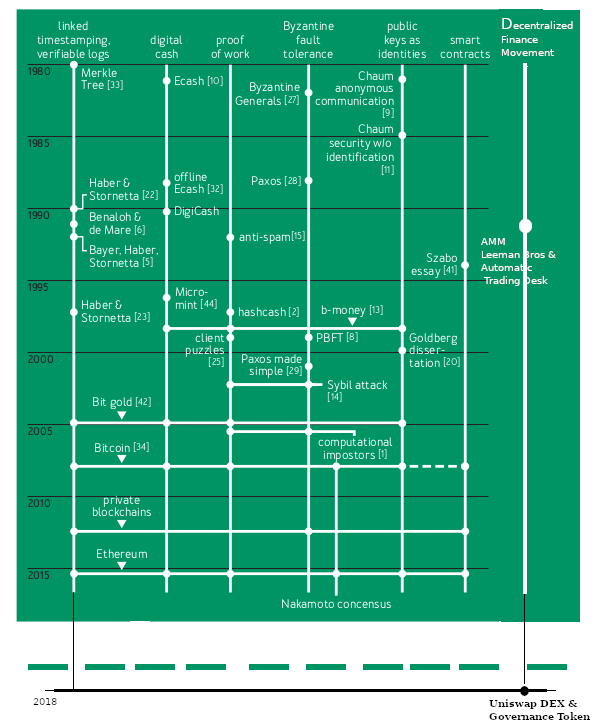
\includegraphics[width=0.38\textwidth]{narayanan3.png}
    \vspace*{-0.3cm}
    \caption{Blockchain key ideas including Nakamoto consensus and DEFI (adapted from Narayaran and Clark, 2019)}
\end{figure}
 
 The Ancient Greek astronomers had defined the logarithmic magnitude system and introduced concepts of limits and infinitesimals that would become the basis of differential geometry, calculus and numerical methods, all readily found today in open source tool-kits or programmable libraries for the development of astronomy, like Astropy.
 
 It is now known after a plethora of multi-disciplinary studies including that of \citet{Freeth2021} that during the decline of Ancient Greece the first analogue `Computer' was temporally `lost' to most of the technological world, and only in the fourteenth century comparable `advanced' mechanisms where developed in Astronomical clock machinery in Europe. 
 
 Now, more than two-thousand years hence, Alan Turin (AT) is widely recognized as a modern father of The Computer for his pioneering  work in the twentieth century that paved the foundations of Artificial Intelligence (AI) and Cryptography. 
 
Cryptography is the basis of Open Blockchain ledger technology, a technology that until now has not been much considered for astronomy development, least as a potential interoperability catalyzing agent. In fact cryptography for Astronomy has only been explored as an ancillary technology for limited communication protocols in astronomy,  data compression, permission and some related data fidelity issues.

Conversely, Artificial Intelligence (AI) techniques like `Machine-learning' and `Data Mining'  have become increasingly relevant for Astronomy as can be measured by the increased number of published studies during the last two decades in astronomy and astrophysics peer-reviewed journals. Some of these studies have estimated the physical parameter space of astronomical sources from large ensembles of data measurements over the observable parameter space and have led to the classification of astrophysical sources and relations or laws that govern The Universe. AI technology is proving fundamental in the so-called data-tsunami era of astronomy through these data-science techniques, partly due to the necessity of mega-survey's optimization of data that must consider: Velocity, Volume, Veracity, and Variety; each of these constraints must be optimally set for specific science-cases. High cadence astrophysics events for example for the study of Kilonova transients require multi-messenger observations that depend on real-time AI alert systems to constrain Kilonova specto-photometric models and have revealed only in the last few years that rapid neutron capture, or r-process nucleosynthesis reactions, produce dense neutron-rich material in the ejecta produced by the collision of two neutron stars, see \cite{artola2020}. Many of these advances have come from direct use of Open Source library packages in Python. These libraries include community developed core packages, for example $\textit{Scipy, Matplotlib, Astropy., etc}$, see Figure \ref{fig:astropy} and affiliated packages submitted by uses. This ecosystem is proving increasingly relevant for the evolution of Astronomy not just because of the ease-of-use of the programming language Python but because of the nucleation of the community development model that minimizes redundancies and gravitates to best-practice procedures and selfless collaborative opportunities. It is argued here that Open Source is likely causal for many of these developments and although a necessity for some collaborative projects may in itself fall short and not be sufficient for others within the domain of Open Development funding in Astronomy, a central tenet of this white-paper. Tsunami data-streams from surveys are not easily accessible for reprocessing in easily public verifiable form and data-access depends to some degree on propriety periods or in-house techniques. An examination of the Vera Rubin pre-processsed survey data is a case-in point. Data from the Vera C. Rubin Observatory, previously referred to as the Legacy Survey of Space and Time (LSST) once observed is pre-processed and ingested into seven Brokers that have all been selected in an open community competition call.  The out-going stream from Vera Rubin has sufficient bandwidth for ingestion of only seven `community Brokers' that have been selected: Alerce, Ampel, Antares, Babamul, Fink, Lasair, Pitt-Google. These teams no-doubt still represent some degree of centralization, since teams are somewhat skewed to different specific science objective, skill-sets and the codes are not optimally community driven. Could DEFI be used to fund a dedicated Astropy community Broker, rewarded via Oracles for software and data analysis? Another example, in the VVV survey, an issue was found in the preprocessing algorithm by a team member that had proprietry access to the data. In Victoria Santuchos Licenciate thesis, `Vicky' determined that the CASU 1.2 pawprint catalogs had systematic magnitude differences due to a 'grouting error' in the preprocessed data (Mike Irwin, priv comm), see FigX. These was able to be fixed in later releases yet most people who used the corrected data are indifferent of Vicky's work. Decentralized Science funding or DESCI via existing governance structures like IVOA \& IAU could be used to address these subtleties of development, mitigate some of their ill-effects and lead to open Astronomy development standards that through Federated learning models and appropriate incentive mechanisms based on open Blockchain protocols could add guard-rails to increase the efficiency of the  ELT (extract, load, transform) processes required. In the case of the Rubin surveys brokers are even responsible for the source-matching. However as has recently come to light in the IVOA-exec, the IVOA itself can not recommend source-matching or even best-practices and so a corollary arises: Could the data-streams use open Blockchain protocols to protect data provenience and unite users across brokers over different wavelengths and AI learning methods, data, and models? In this whitepaper, Blockchain is proposed as this missing link in an environment where the half-life function of US PhD majors in astronomy is in steep decent and where projects are becoming much more reliant on team science and access to new technology development, especially in developing countries becomes increasingly difficult since the burden of the opportunity cost to development is most sensitive to international markets where the fiat cost of technology development is prohibiting.

\emph{Our goal then is to discuss the Bitcoin blockchain standard, and to identify useful elements for a potential base-layer stack for the Open Development of Astronomy including the on-boarding of existing astronomical institutions.}

\section{Blockchain as a corner-stone for Astronomy Open Development?}
\label{sec:bc_review}

As aforementioned see Figure 1, DEFI is much rooted in Open Blockchain protocols including the Nakamoto consensus. Similarly DESCI it is argued is considered to also be rooted in open Blockchain protocols, with the onus that DESCI protocols must set out to advance open science development, managed by the scientific community. Initially any AOD DESCI Blockchain project will likely depend directly on DEFI protocols for seed funding to permit capital in-flows from more general DEFI liquidity markets as determined by DESCI community governance. In the case of Astronomical project liquidity might also flow into more general DEFI liquidity markets (through staking, yield farming, loans, prediction markets, etc), decisions must be strictly determined by governance on a case-by-case basis. Nevertheless success or failure of AOD tied to Blockchain protocols will ultimately and more adequately be determined by the wide-spread use of community developed applications and carefully defined metrics by the community. \cite{arvindandclark2017} point out that the main challenge for wide-spread adoption of decentralized open Blockchain ledger technology lies in its utilization by existing users (and institutions) and not in new users from new blockcahin institutions. If we consider that that growth in modern Astronomy has been driven by hardware and software (eg: CCDs, Python, Astropy etc) development then it may be somewhat surprising that unlike AI, Blockchain as a technology has heretherto not been much considered in the Astronomical literature even though development funds are difficult to come by. Nevertheless bitcoin has been the commodity with the highest ROI in over a decade.  A model heuristic of this white-paper (WP) centres on highlighting this discrepancy and proposing solutions, in the context of the data Tsunami Era, one in which collaborative mega-projects require use of so-called Public Astronomy Brokers \cite{bellm19} as open as possible to community development.  

It is noted that the conservation of the M2 money supply is not time-invariant like are other fundamental physical constants in The Universe since it depends on central bank issuance through highly centralized institutions like the US Treasury and Federal Reserve as well as similar institutions in other Nation States and other levels of  government that are often related. Sound money on the other hand as a concept is more akin to principles of Austrian Economics and although is somewhat beyond the scope of this paper sets some fundamental constraints on open Blockchain ledger technology, the subject of this whitepaper. 
DEFI and DESCI are self-consistent ideas that depend on smart-contract automatic market making technology (AMM) to facilitate token swaps and other more complex transactions without third party intervention (eg: NFT royalty payments) via DAPPs through (1) Decentralized Exchanges (DEXs) like (2) `UNISWAP' etc. UNISWAP is chosen fiducially because it is the first DEX to offer a massive governance `airdrop' that to-date maintains a large fraction of the total locked Total Value (TVL) of all DEFI protocols. \footnote{\href{https://defillama.com/protocols/dexes}{DEFI LAMA}}. The Uniswap treasury has more the 4.6 billion USD in TVL.   Nevertheless, DEFI that sets to overcome the pitfalls of centralized banking and financing in different industries was already a central tenet of the Nakamoto Protocol as referenced in Bitcoin's genesis block \textrm{coin-base field} \href{https://www.Blockchain.com/btc/tx/4a5e1e4baab89f3a32518a88c31bc87f618f76673e2cc77ab2127b7afdeda33b}{HEX to ASCII}:  'The Times 03/Jan/2009 Chancellor on brink of second bailout for banks' \footnote{https://hackernoon.com/chancellor-on-brink-of-second-bailout-for-banks-where-to-find-this-on-the-bitcoin-Blockchain-hm4k34v4}, and in emails and reply's by Satoshi to the cyberpunk's mailing list, that relates energy and time or Power in a transactions based system, examined more thoroughly in Section \ref{sec:energy}.

\subsection{Review of Blockcahin primitives and Key-Ideas}
\label{subsec: review}

\cite{arvindandclark2017} show insurmountable evidence as do other authors therein that standard open Blockchain protocols are much rooted in academic studies of cryptography. Fig \ref{fig:narayanan} is an adaptation of fig1 of \citet{arvindandclark2017} with the addition of a key-idea or related notion: The Decentralized Finance Movement or "DEFI" that through a `non-custodial' or decentralized exchange "DEX" may issue governance tokens to fund open development incentive efforts. There is much evidence that DEFI was already implicit in the Nakamoto consensus from the outset. As a notion it is referenced in the white-paper as in the `cryptographyat metzdowd.com' mailing list emails from Satoshi in October and November 2008, and in the bitcoin genesis block. In any case a DEX permits automatic market making (AMM) token swaps providing incentive fees for liquidity providers. Nick Szabo first proposed `smart-contracts' as a Blockchain primitive in Extropy #16 . This term is unrelated to AI but more related to automatic P2P transaction conditioning that does not even require human intervention. Alice and Bob can be machine and machine!  In any-case a `smart-contract' can be automatically executed in the cloud on a "trustless" financial rail system like the Bitcoin network. The transaction (Tx) contracts via 'non-custodial' community built infrastructure will automatically be executed prohibiting at the protocol level any interference of any third party. Initially developed to omit the need of a centralized order book, a DEX should minimize other counter party risks to contract execution, for example web Framework server failure, like that suffered by INFURA Denial-of-Service (DOS) attack to its price Oracle which unpegged US stable coin values that incurred million dollar losses in Dec 2019 to the Compound protocol, so caution of infrastructure selection must also be strongly contemplated by the Astronomy community. Following Szabo's definition, \href{https://www.fon.hum.uva.nl/rob/Courses/InformationInSpeech/CDROM/Literature/LOTwinterschool2006/szabo.best.vwh.net/smart.contracts.html}{Smart Contracts} could integrate into base-layer applications like Oracles to automatically in-jest data from third-party data-feeds like NASA ADS publication metrics within a research subject, field, key area,  or even institution. All counter party risks must be averted in contract-design if true decentralization is to be met. Governance through voting must also be thoughtfully contemplated and implemented. Note:  More detailed on DEX can be found in \cite{uniswap2019_angeris} who explore technical details of Uniswap and its use as a financial DEFI source.




\begin{figure}
    \centering
    \label{fig:astropy}
    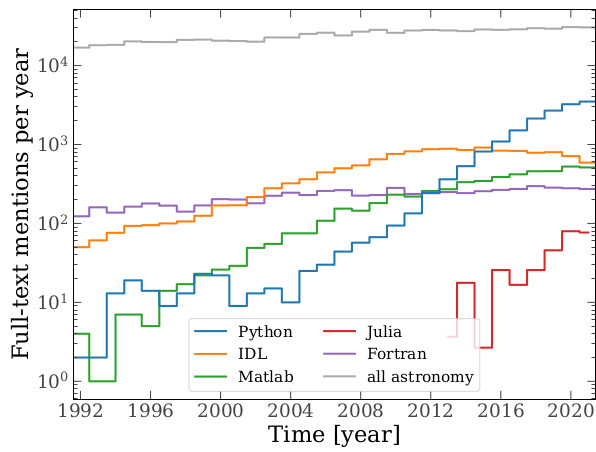
\includegraphics[width=0.38\textwidth]{figs/2206.14220.jpg}
    \vspace*{-0.3cm}
    \caption{Reproduced from Astropy Core paper showing Full-text search for 'programming language' returned query in NASA ADS}
\end{figure}

 \begin{figure}[h!]
    \centering
    \label{fig:cowen}
  \caption{Historic Price (USD) function of BTC in time (Years), as an underlying store of value for Astronomy Open Development (AOD). The figure includes a color-bar risk metric as modelled by Cowen et. al; (2021) for 3 prior market-cycles that have been identified by Cowen to have been dependent on the bitcoin block reward halvings, every 210,000 blocks.}
  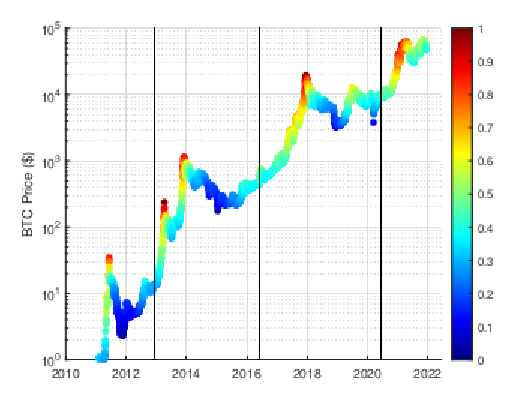
\includegraphics[width=0.5\textwidth]{figs/cowen2.eps}
\end{figure}

\begin{figure}[h!]
    \center \begin{figure}[h!]
    \centering
    \label{fig:cowenbtc}
    \caption{Historic Price function (in USD) of BTC in time (Years), as a potential underlying store of value for Astronomy Opem Development (AOD). The figure itself and color-bar risk metric is as modelled by Cowen et. al; (2021) for 3 prior market-cycles that have been identified by Cowen to have been dependent on the bitcoin block reward halvings, every 210,000 blocks.}
    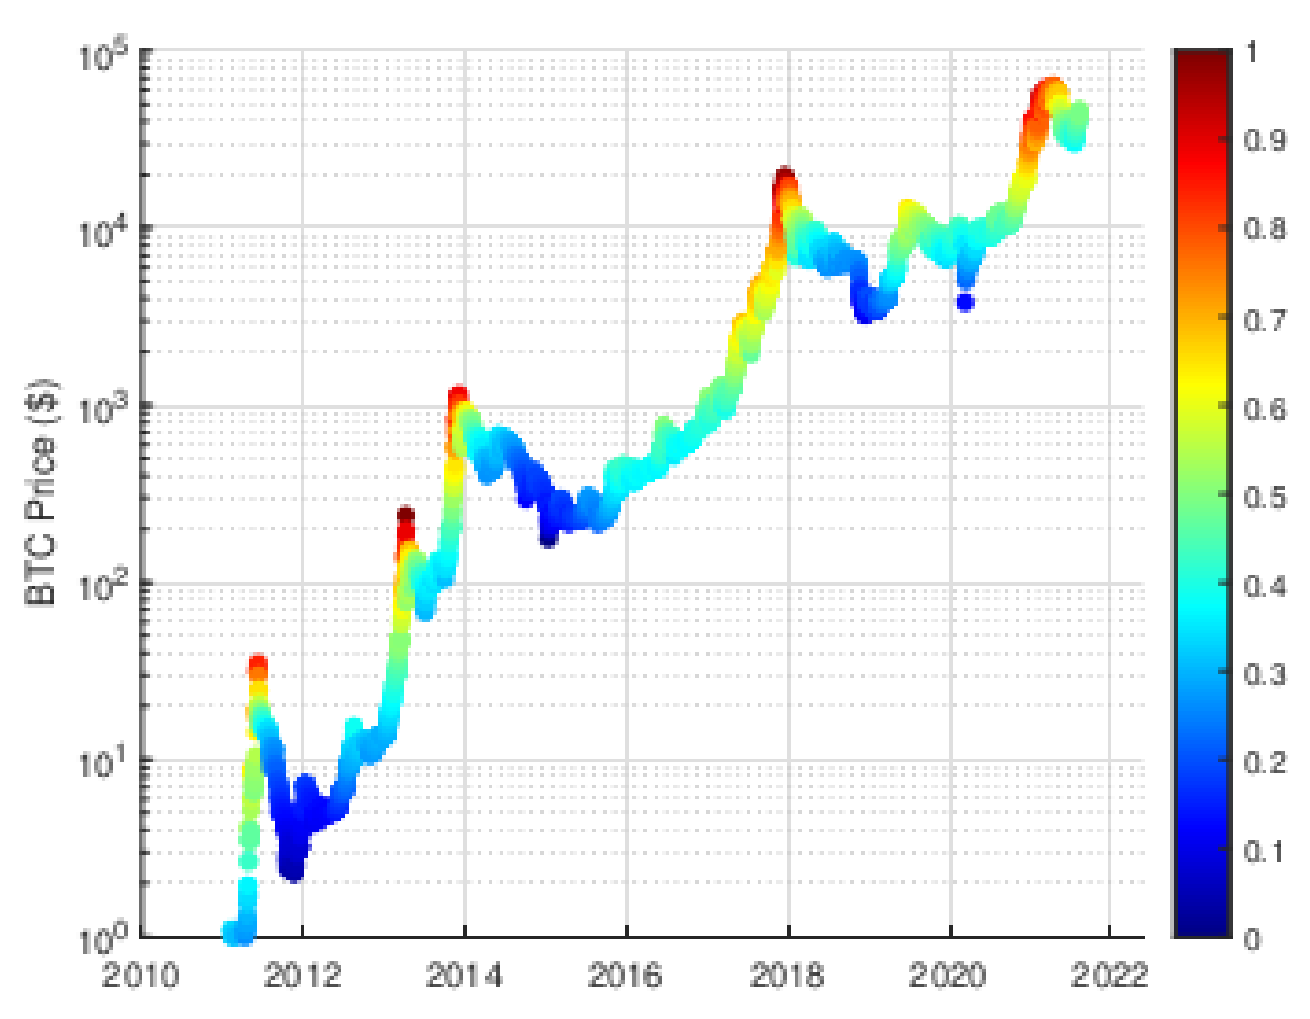
\includegraphics[width=0.5\textwidth]{figs/cowenbtc.eps}
\end{figure}

\begin{figure}[h!]
    \centering
    \label{fig:crisis}
  \caption{Historic global Crisis, Figure taken from \href{https://en.wikipedia.org/wiki/Global_recession}{wikipedia-commons} adapted from data Reinhart and Rogoff (2009) depicts the binned instances of global crisis (Y-axis) for individual countries that grew in number exponentially before and after the US Nixon administration pulled out of the Breton Woods accord unilaterally that required physical gold backing to USD money printing.}
  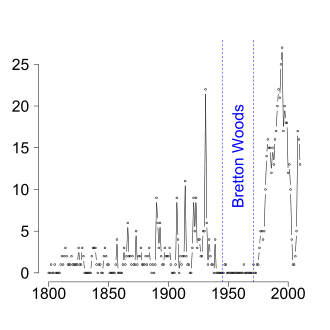
\includegraphics[width=0.5\textwidth]{figs/330px-BankingCrises.svg.png}
\end{figure}

\begin{figure}[h!]
    \centering
    \label{fig:F4.large}
  \caption{Figure taken from Milojević et al.) depicts the falling half-life rate in Astronomy and Astrophysics and other STEM fields}
  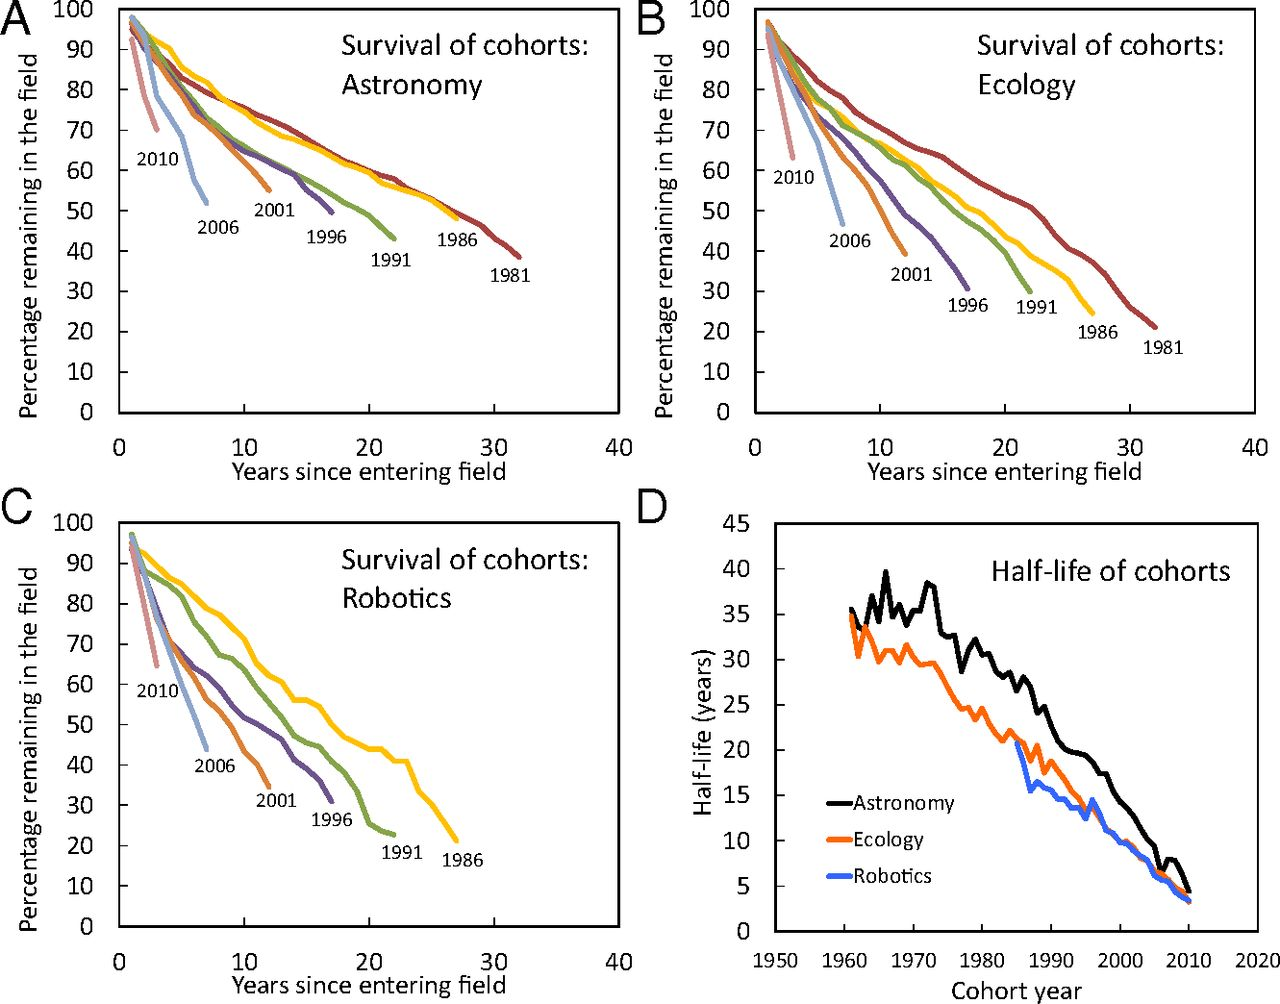
\includegraphics[width=0.5\textwidth]{figs/F4.large.jpg}
\end{figure}ing
    \label{fig:crisis}
  \caption{Historic global Crisis, Figure taken from \href{https://en.wikipedia.org/wiki/Global_recession}{wikipedia-commons} adapted from data Reinhart and Rogoff (2009) depicts the binned instances of global crisis (Y-axis) for individual countries that grew in number exponentially before and after the US Nixon administration pulled out of the Breton Woods accord unilaterally that required physical gold backing to USD money printing.}
  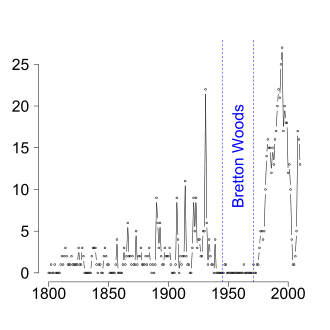
\includegraphics[width=0.5\textwidth]{figs/330px-BankingCrises.svg.png}
\end{figure}

\begin{figure}[h!]
    \centering
    \label{fig:F4.large}
  \caption{Figure taken from Milojević et al.) depicts the falling half-life rate in Astronomy and Astrophysics and other STEM fields}
  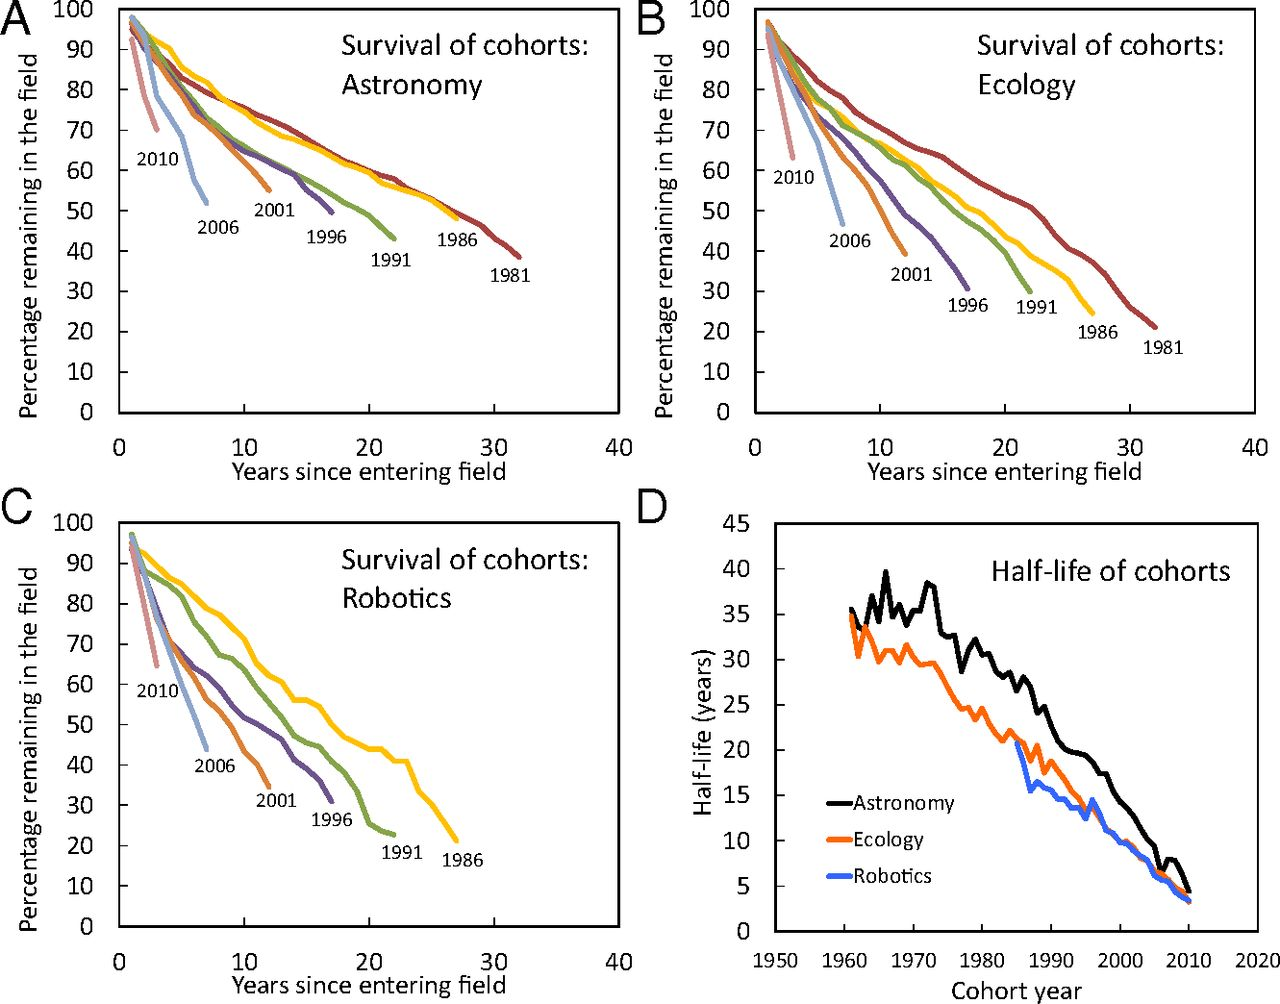
\includegraphics[width=0.5\textwidth]{figs/F4.large.jpg}has in order to be a
\end{figure}
This paper starts out by assuming the Nakamoto Blockchain Consensus from the white-paper of \cite{nak2009} and subsequent Bitcoin Improvement Proposals (BIP) form a base layer store-of-value for AOD. Although the Nakamoto WP was first published in Cryptography mailing list, there is much evidence that ideas were discussed in CPunks, during the 90s; by leading academics. A review of the Bitcoin standard and its relation to Austrian economics can be found in \citet{Hansen2020Book}. Suffice to say, Bitcoin is the first global financial anonymous network with the following key properties: its proof-of-work consensus algorithm makes it highly secure resistant and resilient to attacks, it perhaps the only crypto asset that is labeled as a commodity and not a security amongst regulator bodies worldwide. It has remained since its inception the Blockchain with the larget market-cap bar none. It includes a block-size constraint that allows full-nodes to be run even on a single PC. Its supply function is capped at $21\,000\,0000$, and new blocks dependent on miner rewards and two-week difficulty adjustment, as well as other technology incorporated over its history of life via bitcoin improvement proposals (BIPs). It uses POW for mining. It has proved to be a valid store-of-value with an ROI far superior to the USD and Gold. Although as noted, on short time-scales, (less than a few year) the BTC price (in USD) is highly volatile, on-chain analysis indicates that over time volatility is decreasing yet the BTC/USD is still much correlated to global financial markets (Lyn Alden) and hence inherent volatility yet on longer time-scales BTC volatility as measured by Cohen et al. and other authors is falling until monetization which is likely to occur in the next two cycles (approximately 6 years), when BTC total market cap is expected to overtakes that of gold. 

The latest L2 BIP update occurred at the end of 2021 and includes smart contract capability through the TAP-ROOT extension that has made the network more scalable (to get around the limitation of the 10-min average block node confirmation), and the earlier Lightning BIP built necessarily on-top of Segwit, is more than enough for smart-contract Tx requirements for AOD applications nevertheless other, less secure open Blockchain protocols as mentioned  offer advantages in funding and fuctionality including scalability and Tx costs. Market cap, ease of use, developer numbers, technology standards, cross chain metric analysis, as well as other indicators for other L1 chains must be considered including Ethereum, DOT, and perhaps other chains. Many of these alt chains have helped in the technology development of Bitcoin network. The LTC group of core-developers for example have helped develop Lightning. Many alt L1 have thriving developer communities, DApps and billions of USD in locked liquidity and are part of the burgeoning Decentralized Finance Movement, whose primitive protocols may offer advantages for AOD and seed-funding from DEFI grant funds, that may all help seed AOD for Astronomy. 

Section \ref{sec:use-case} is an attempt at an institutional map of the Astronomical Observatory of Cordoba/IATE. Blockchain dinamics are conisdered for its various sub-units departments, research groups, programs, educational, academic etc., functioning including "Telescopio Itinerante", "Noche de los Museos", "Museum del Observatorio Astronomico", "Library", "FOF workshop" as identified. The IATE-OAC has over 80 staff including permanent academic staff, graduate and undergraduate students,  CPA (Technical and auxiliary staff) all which make up an otherwise thriving ecosystem. It is argued that for successful open protocols in Astronomy, incentive system must be worked-out within these units of existing institutions to allow for liquidity partitioning to direct to Open Development despite otherwise hindrance in funding challenges given the existing system of funding.

%Smart contract first coined by Nick Szabo have nothing to do with AI but instead related to the concept of automatic conditional P2P transactions that obviate requirement of a third party that may more often than not be a centralized entity. Smart contracts may be  automatically executed by one or several parties. According to a \href{https://www.fon.hum.uva.nl/rob/Courses/InformationInSpeech/CDROM/Literature/LOTwinterschool2006/szabo.best.vwh.net/smart_contracts_2.html}{community vetted smart contract protocols} are useful data-stuctures for open Blockchain development that have applications including Oracles that could involve tokens and nodes that validate transaction and receive data from external data feeds. These could be useful to adjudicated resources using community established metrics that may include publication rate in international refereed peer-reviewed journals or as  a research subject or field, group or institution, including macro metrics like GDP increase towards science and development could be taken as  valid metrics. 

Governance protocols based on smart-contracts are identified as part of potentially successful AOD infrastructure, since the voice of the community may be efficiently enacted  actions decided via voting etc; Prediction market protocols could also be used to help AOD mitigate against stochastic ill-effects that may cause restrictions to Open development caused by other status-quo 'hard-wired" funding mechanisms. For example in Section XXX we examine the TFlop computational issue facing Argentine Astronomers (mostly N-body, and Grid), in which HPC Argentine Research Scientist are at a disadvantage since TFlop capability as much technology is priced in USD. So delays of years to obtain project money to start building HPC infrastructure put Argentine Astronomers on an uneven playing-field. In Fact, it was stated in the Jornadas de Computation de Astronomia de Argentina (Nov 2021)  in which the IATE invited members across all the astronomical institutions to discuss these issues in a workshop, that pooling resources is necessary but not sufficient because of rising capital costs to UPC, air-conditioning, rising energy costs, network core infrastructure costs, so research projects often have to be scaled back in response to these elevated costs or depend on external  collaborations and infrastructure. In Figure \ref{fig:crisis} we reproduce the historic global crisis function of nation states that depicts an exponential increase in crisis instances during periods when `sound money' was  unfamiliar to most governments of the world. It is concurrently noted that these periods affected and retarded astronomy open development since in those times more essential funding priorities dominate including using available funding to cover the bare essential necessities of the population. We emphasize from this figure that during the Bretton Woods accorded period, or the period within the de-marked broken blue lines that the occurrence of financial crisis was approximately a global minimum. 

Could the Nakamoto consensus as the go-to store of value or sound money base protocol and subsequent BIPs usher-in a new period of stability and even innovation for OAD in Astronomy? 

In Fig 3 we reproduce the empirical half-life function for astronomy and astrophysics PhD majors as well as other STEM fields within the US Public University System. It is clear that this figure is shows alarming exponential rate of decline.  In this section we have discussed the current and historical situation that has underpinned the negative effects of Astronomy development with examples. Some Blockchain primitives and protocols are identified, selected to complement Open Astronomy Development.  In Section \ref{sec:btc4} a simple idea of implementation and on-boarding for our model of Astronomy education/development and research via open development is proposed via Astropy, the leading Open Developer community tool-kit by Astronomers for astronomers. In Sec. \ref{sec:btc5} conclusions drawn and some discussion on a possible future course of action plus an NFT case-study to celebrate 150 years of the Observat\'orio Astron\'omico de Cordoba, the former National Argentine Observatory. 

\subsection{Early Blockchain Fundamentals}
\label{subsec:fundamentals}

The Turing complete programming languages like ETH (#reference to Anonopolous ETH book) have loops and are able to iterate infinitely and have central actors (Founder, Cofounder, VC-funds, etc). Bitcoin on the other hand is Turing incomplete, purposely built to be much simpler, it has proven over a decade (see Fig \ref{fig:btc}) to be a excellent store of value when compared to the USD over time-scale of a few years. Advanced Smart Contracts capabilities were never part of the immediate scope of the original implementation. Whereas Bitcoin was primarily designed to be a P2P form of electronic cash, other Blockchain light Litecoin where used to test implement the Lightening network and other technological complex smart contract capabilities. For example the Ethereum Blockchain has shown itself to be a successful Blockchain for more advanced smart contract capabilities, and has been defined by its lead developer to be a “World Computer”. There are many excellent sources in the Literature on this topic, suffice to say that Bitcoin devs with BIP XXX YYY have implemented advanced smart-contract cababilities on layer 2 and that below we will concentrate on atributes of a Token for Astronomy choosing a hybrid approach based on ETH and BTC liquidity in the Section below in which we describe aspects of our Astronomy OD model.
 

Preceding BITCOIN, many advances in Blockchain technology were made in works like Chaum (1983), Chaum, Fiat Naor (1989), Rivest and Shamir (1997). Haber and Stornetta in 1994 building from the literature as well as from their own paper in \cite{Haber1991wi} put a Pulic Open Blockchain system into practice in the New York Times classified. This being the first accredited ledger that was a digital signature time-stamping validation service named "Surety", fourteen years prior to Bitcoin. 

However the first decade of the 21st century gave rise to perhaps the most famous Blockchain system, the Bitcoin standard, published anonymously by Satoshi Nakamoto in 2008.  In the first block, see Figure X: Satoshi made reference to the New York Times article that reported that the then U.K. chancellor was considering a second Bail-out round of the largest UK Banks. Satoshi, probably a pseudonym is demonstrated to have been from the academic literature since Satoshi much cites the academic literature. That according to some analysis may represent the work from mostly one individual (MOOC Blockchain, Princeton), although definitive evidence remains somewhat elusive perhaps more evidence will come to light if the early Wallets of Satoshi that contain many early Bitcoin become active. Moreover the identity of Satoshi or any Blockchain OG is a surface of attack to that network so it is no doubt that Satoshi identity is hidden by design. Never-the-less Bitcoin and it's Blockchain network and bitcoin the asset has grown in value more than any other asset classes, including gold, so it could be argued that so far, in the time-frame of years in it's first decade of existence the Store-of-value proposition appears hold.

In shorter time-frames ($\lt \sim 1$ year) BTC volitility is significantly higher. No doubt compared to other asset or commodity clases like Gold it is measurably young and hence volatility high, since if it is to represent a global commodity reference, its market cap will no doubt be more sensitive to external speculative financial capital markets. Energy Usage is also discussed here in Section \Section{energy}. 
 
BTC as a world reserve still appears to be partly correlated to other global financial markets. A recent example is the Covid19 black Thursday pandemic that in March 2020 saw BTC price drop by more than 30\% in only a few hours. This appeared to be triggered by the Black Thursday liquidity crisis that swept the much larger global financial markets and the reactions of central bank governments to it as did the Omicron crash of December 2021. The March 2020 crash coincided with a crash in global equity markets that saw stocks suffer the worse losses since The Great Depression" and iconic corporations were "bailed out", like Hertz after a record number of unemployed, filed for unemployment benefits in the US. After about a fortnight, like many blue-chip stocks, bailed out by the US FED via Repo, corporate bond offers, and share buy-backs the BTC recovered almost instantly. Against other asset classes including gold and USD, BTC appears to be in the short scales at worst, as volatile. 
 
Bitcoin as a technology to solve several problems faced by earlier digital currencies. Having no single point of failure meant law suits can not be used to persecute anonymous creators. This adds to network security by processing Hash functions which is adjusted on a two week basis. Some authors, including Andreas Antonopoulos believe Bitcoin and Ethereum Blockchains have the potential to revolutionize open development in science and technology and with 5G roll-out promise unprecedented levels of growth of over 18 percent per year, not seen since the first industrial revolution Waldon, M.  Fig needtoinsertfigure adapted from Walden et al. shows the world GDP as a function of time. These technologies were born out of academia, the occupy wall-street and anonymous movements as a direct response to the 2008 financial crisis that saw a global slump in the world GDP based on the US sub-prime financial crisis  that included a drop in US GDP by 30 \% sustained over several years.
 
Programmable money is not exclusively relevant to human beings but also to machines as participating actors. Hardware evolution is also tied to open development, as seen in the evolution of specialized hardware architecture for Proof Of Work (POW) HASH Function calculations that is developing Application-Specific Integrated Circuit (ASICS) to mine Bitcoin blocks. It could be argued that these developments have outpaced Moore's law.  Wrights Law suggests that the for every percentage increase in the cumulative distribution function of production in any industry equates to a fixed percentage increase in the efficiency of production. So hardware has evolved from CPU intense through to graphic processing units (GPU) and  Application Specific Integrated Circuit  (ASICS), \cite{10.1371/journal.pone.0052669}. A successful model for Astronomy and Astrophysics Open Development would do good to tie metrics of Open Production into the protocol as well as the appropriate incentive mechanism.       

Open Blockchains are uncensored so a data protocol standard of best practice through governance could be cross validated from an information criterion perspective that includes Oracle feeds for Open Development.  Oracles that receive feeds are penalized if they predict incorrect probability distributions of events or Facts for Astronomy Development prediction markets. 

\section{Energy and Bitcoin}
\label{sec:energy}
The Bitcoin network has been criticized for the Power required to operate and secure it. This Section attempts to examine the Energy use of Bitcoin from an astronomical perspective by comparison to the Kardashev \cite{kar64} scale. Bitcoin hashing is considered fundamental to the POW protocol for the: (1) production of new blocks, (2) processing of unspent transactions (UTXO). At any time, the hash rate is a measure of the hash-power of the total Bitcoin POW system.  


\subsubsection{POW Incentive}
The target hash-rate for Bitcoin is a moving average of the hash rate over the last 2,015 blocks.The hashing power is estimated from the number of blocks being mined in the last 24h and the current block difficulty, given the average time T between mined blocks and a difficulty D, the estimated hash rate per second is given by:

$\textrm{H} = 2^{32} \textrm{D} / \textrm{T}$

Considering that roughly every 10 min a new block is minned, so 2015 blocks represents nearly a perfect two week interval. This is the difficulty adjustment time-scale. In actual fact, a bug in Satoshi's Bitcoin Core client code or a zero-error=1 persists, such that the the first block of every 2016 blocks post adjustment, is not actually included in the moving average calculation, only the last 2015 blocks are used. This bug can only be changed with a hard-fork, a cost to date, too high for the Bitcoin core devs. Now, given the instantaneous hash rate will depend on many variables like seasonal electrical supply cost, technology developments, miner adoption, etc., miners may temporarily switch off mining units. For example, in Southern China in the Summer months the monsoon Wet-Season provides abundant energy supply that drives more intense miner activity such that the total China hash-rate committed may increase by more than 100 \%, with electricity generated from stranded hydro facilities (REF). Nevertheless, on the criticism that Bitcoin Network requires as much power as some Countries like Argentina or large cities as New York, confusion is often and unwittingly made between Energy Consumption and Energy Production. The Bitcoin energy consumption models by the Cambridge University Judge's University Center for Alternative Finance or simply the Bitcoin Energy Consumption Index has been used to tie to some early Astronomy models in searching for insight. The Bitcoin Energy Consumption Index estimates the Energy Consumption by modelling the Bitcoin hash rate with hash computes using a Normal distribution of basket miner technology (GPU's, ASICS etc), taking into account technological advances in Hash Computes, World Energy costs ., etc. Using all model parameters the CBECI estimate that as percentage of world total energy for Bitcoin will remain below 0.1 \percent for its lifetime. Other authors like Antonopoulos argue that the energy cost of the Bitcoin network is near the noise of the total energy consumption yet it may be a necessary cost required to secure a reserve global decentralized and uncensurable financial network. Although full Bitcoinization is speculation in this section we start out considering two canonical papers on the subject of Energy consumption for technologically advanced civilizations by Kardashev 1964 and Sagan 1973 and then adjust these models for Bitcoin Hashrate and make a plot in Fig XXX to visualize the evolution of power for Bitcoin over a x year base-line taking the Cambridge Bitcoin Electricity Consumption Index, Bitcoin Use Scale as predicted by . 

$E_BTC/E_tot < 0.1$

More than just the production of new blocks or new bitcoins, it must be recognized that (i) this cost is to secure the network (ii) energy consumption and energy production are two different concepts that must not be confused (iii) a significant percentage of POW hash-rate is powered by renewable energy sources that this Bitcoin Network could be updated if desired by miners, holders and the general community, on renewable and sustainable stranded energy or carbon credit system. Of course on the topic of energy consumption, the \cite{kar64} model or Energy Use function for civilizations is a useful comparison chart to ascertain the current Energy situation of Civilization on The Earth over a longer bast-line of time to mitigate a type of recency bias, and given the potential of wide-use of Bitcoin adoption, we analysis this in this paper. In the \cite{kar64} equation 1:

\begin{equation}
    (1+x)^t \approx e^{tx}
\end{equation}

Kardashev estimated that with an average sustainable increase of 1 \percent per year energy consumption Humans would reach a Phase 1 civilizations and able to use all energy incident on the home planet (Earth, for us Humans) from its parent star, and Phase II reach the capability to use the Bolometric Luminosity of The Sun of roughly 3.9 X $10^{26}$ W. see Table 1. Incidentally, this is in-line with Wrights law as  discussed above. \cite{Sagan73} re-define the zero point of the scale and formalize an information metric that Kardeshev originally contemplated to accompany the energy metric or binary tree and show that to discern all the information of the then Earth including Greek Philosphy, one would be 2**16 bits. Table one shows the predicted Energy Consumption by advance civilisation from Phase I to Phase III, based on \cite{kar64}. We plot these values in the Figure  used to predict the year that the Earth's civilization could reach Phase III in our hybrid model, given Bitcoinization and the extrapolation of Global Energy Usage we assume Bitcoin value-layer to also be locked t Global Energy Supply, so we take the zero-point or fiducial point of phase I to Bitcoins 2009 genesis block and phase II to be when the block reward halfing is from CBECI to  estimate that currently the Earth's Civilization is about 2-3 orders of magnitude from reaching phase 1. In \cite{Sagan73} alternate information metric a model is made on the information richness of any civilization. This can be represented in a Binary operations even a Binary Tree which share the Hash Function Structure. Interesting, the Bitcoin Network Ledger which contains transaction information of every single Bitcoin transaction may also be used between non-humans. This may be the sense of "Smart Contracts" by Nick Szabo. The Bitcoin Hash function could be taken to represent a function that could be a proxy for both the Energy Use and the Information in our model. We take data complied from the International Energy Agency and BP, from \ref{owidenergy} and plot the total yearly power production avalable for The Earth. In Fig \ref{fig:kardashev1}, we show the data since 1964. Interesting the last data point is from 2021. There was about a 5 percent increase in production since the 2020 which was the COVID-19 pandemic year.

\begin{figure}
    \centering
    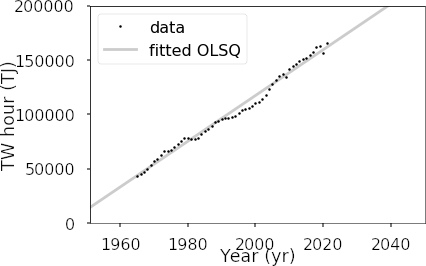
\includegraphics[width=0.5\textwidth]{figs/fig1_kard.png}
    \label{fig:kardashev1}
    \caption{This is the Global Yearly Energy TW hour production metric, taken directly from the Owidenergy resource, with a Ordinary Least-squares fit in Linear scale. The Scipy Python module was used to do the linear fit.}
\end{figure}

In \ref{fig:kardashev2}, we show the same data on a log-log plot and include the Kardashev and Sagan Type I, Type II and Type III civilizations as well as the Solar Insolation Value or the total energy per hour that is absorbed by the Earth from The Sun. 
\begin{figure}
    \centering
    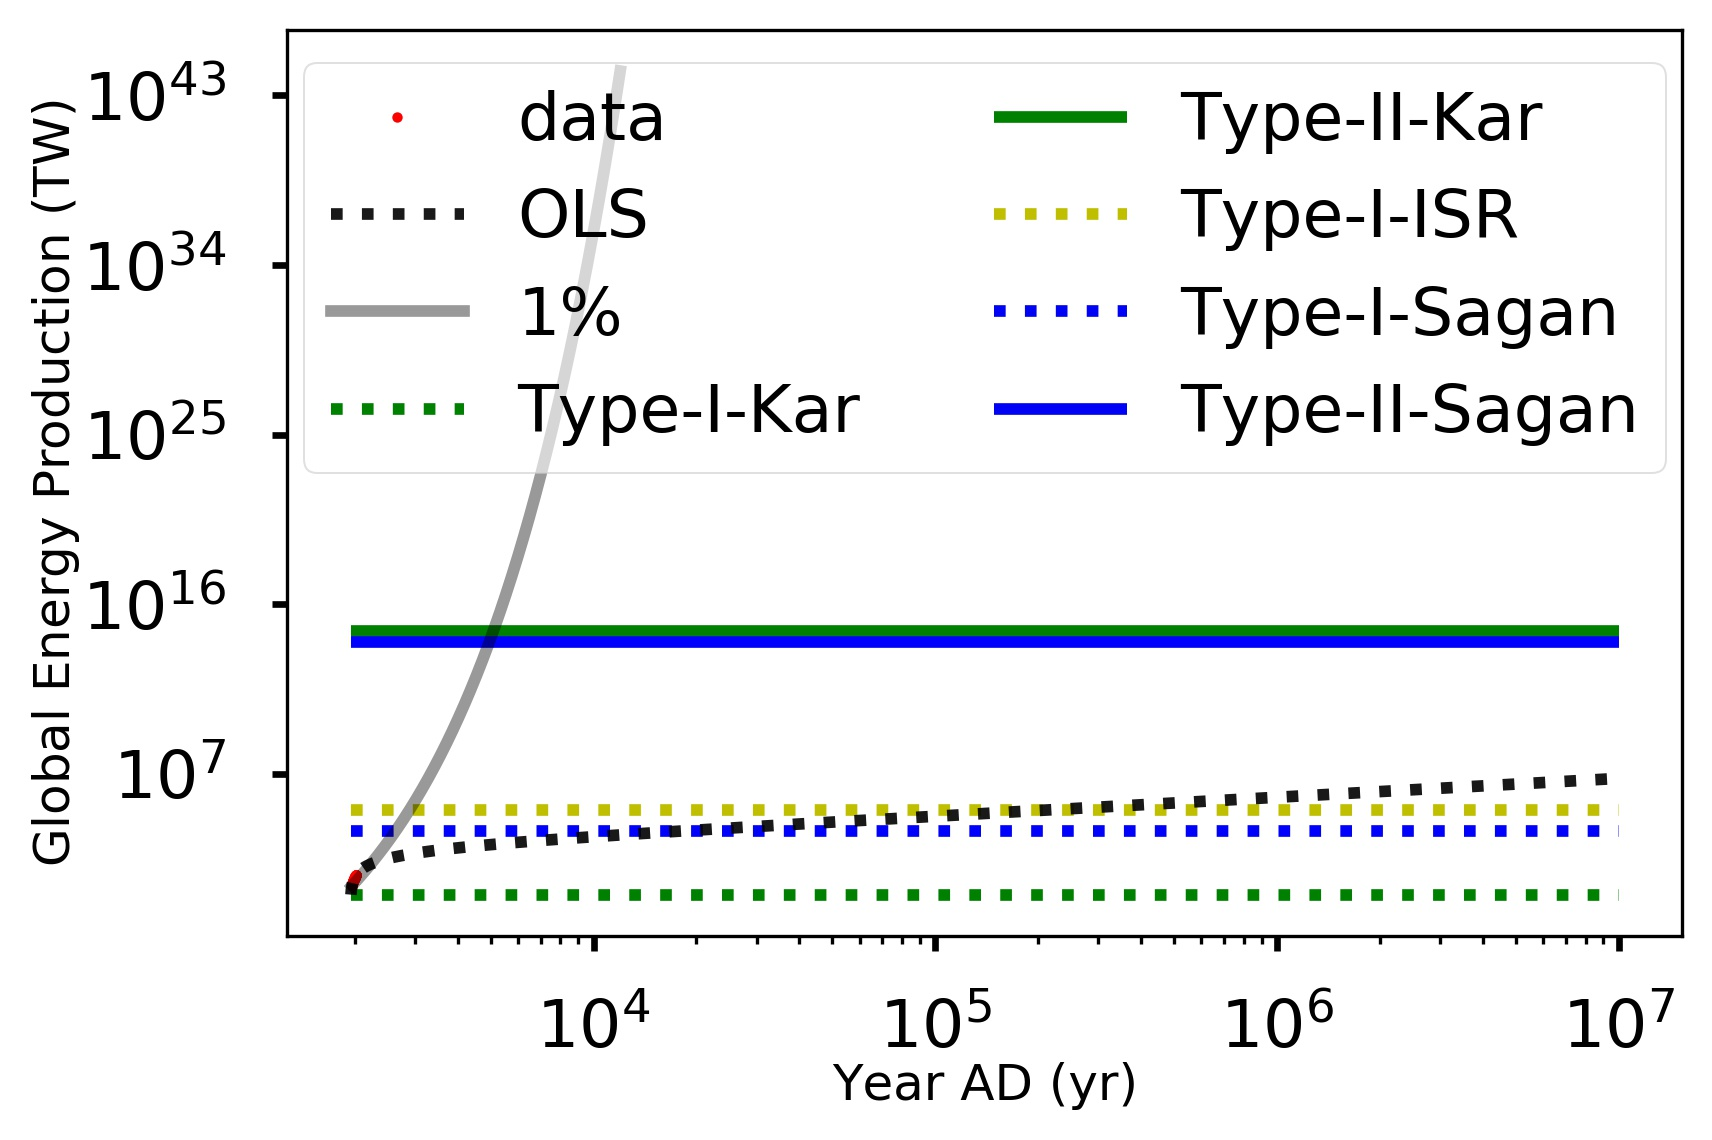
\includegraphics[width=0.5\textwidth]{figs/fig2_kar.jpg}
    \label{fig:kardashev2}
    \caption{This is the Global Yearly Energy TW hour production metric, taken directly from the Owidenergy resource, with a Ordinary Least-squares fit in Linear scale. The Scipy Python module was used to do the linear fit.}
\end{figure}

\subsection{Indexing Open Production and Development}
\section{Open Astronomy development}
\label{sec:btc4}

In this Section we propose five use-cases for Blockchain as case-studies. Chosen across a wide base-line of variety for Astronomy development at the OAC-IATE identified as infrastructure for (i) funding of a new telescope-system TOROS at an ELT tested site, (ii) 'telescopio itinerante' or itinerant telescope program of the OAC, (iii) re-value historical OAC patrimony, (iv) grant stable coin liquidity pool for granted research projects, that is PICT-PIP, (v) Broker for backend of Vera Rubin Survey. 

Although case-types identified mostly focus on  the OAC-IATE, due to more generalized systematic crisis in funding that affects OAD at the global scale so in this context in this section some global salient issues are also examined, including the so-called global brain drain or haemorrhage afflicting astronomers. In Subsection \ref{btc2:sec:sub:half} proxy metrics for AOD are proposed that might go someway to restore historic half-life rate function of Astronomy PhD majors in Public US Universities and associated AOD systems as considered. 

Vera Rubin Surveys 10,000 alerts provided every 39 seconds. Need short time-scale science. Semantically rich alert. Triggering Difference Imagine source, 82 KB per alert means 5 GB per s per full stream. Sixty Second from read-out information needs to get to the Broker system, at least 5 full streams to alert brokers.   For example  Jakob Nordin of AMPEL, requests from the community a standard processing framework for Legacy Very Rubin data, a standard that would enable processing of data-sets irrespective of broker identically and as efficiently as possible, at the moment this is a challenge.  Mathew Graham of Babamul considers that traditional approaches to handle event streams are sub-optimal and sees for back-end work a decentralized network of low-cost components employing commodity AI accelerators and reusable models plus an in-use science data platform for information management that any group can set up on their own at-scale broker for less than 1 USD per day, using Raspberry PI + USB TPUs (4 TOPS), optimal for deep learning models.  Federated Learning for example, which is what Babamul devs have claimed is completely open sourced, could well complement open block chain protocols implementation. Several issues exist for federated learning systems including single-point failure type issues, but also a suitable incentive mechanism to mitigate against data falsification. Blockchain-enabled federated learning can solve these issues as described in 


\subsection{Half-life function}
\label{btc2:sec:sub:half}

The exponentially falling half-life function for Astronomy majors in US public universities is an alarming metric. It is now about 3 years and has been dropping exponentially since about 1970 or about the same time the US withdrew unilaterally from the International Bretton-Woods accords that tied the 'price of one USD' to an allocation of gold. The desertion PhD function could be considered a global hemorrhage of 'grey matter' or capital flight away from astronomy open development.

\emph{In an open development model scientific contributions from the community should be guaranteed, valued and enhanced in a P2P application-layer sense via a more robust gold2.0-standard programmed by the community through open governance Blockchain protocols.}


\subsection{The Merging of Open-Source protocols}

Both AI and Blockchain cryptographic come from Open Source community and both may actually be necesary for the evolution of Astronoomy. To help resolve the issue that is presented by the Data Tsunami, on building deep learning models for large data streams, brokers are necessary, and must be as efficient as possible. For surveys like the Vera Rubin the tasks are complex from cross matching to managing to the community deep learning models to test and refine. Data-rights proprietary periods although have been dropping over time and are now around 6-12 months obviously provide science-team members with a considerable time-sensitive advantage and know-how first mover advantage.  Given the scenario depicted in \label{btc2:sec:sub:half} of increasing number of astronomer PhDs within larger team projects, and considering as reported by the Bambanunu broker team, for deep federated learning decentralized computer infrastructure is expected to be more ideal than large centralized data-centres for many types of problems.  Astronomers that don't have access to such infrastructure to train a models either with their own machines and drawn know-how or are not part of a federated deep learning model will find it more difficult to stay competitive. Blockchain technology could help here too in incentivizing colaboration.   

How to merge Open Blockchain technology to Open Source academic/(community) stack of astronomy protocols via the: Nakamoto Consensus?

In the last decade Open-Source projects in Astronomy have burgeoned and become somewhat unified. 'Astropy' with its community affiliated and coordinated packages has become the leading community repository mine.  One of the reasons the community got behind one project was that many packages offered similar functions and the maintenance costs scaled with the number of version. Some methods may have been more optimal, so a standard system evolved that now maintains the code-base in the community. In Astropysics and other early python repositories for Astronomy the developers recognized with other members of the community that community maintained code repositories was key to development of Open-Source software.

It is contemplated in this White Paper perhaps some-what heuristically that like The Computer that has continued to be a fundamental tool for astronomical problem solving, Blockchain that is itself derived from open source community efforts warrants a more complete analysis by the comunity for AOD. Although most astronomers use Astropy amongst other tools, no block chain modules yet exist on Astropy so we on balance of a community coordinated or affiliated package, consider AstroOD as a coordinated package, since interoperability of coordination is required with other actors and agents of facilities including the IVOA 
\subsection{Liquidity Tooling}
\label{btc2:sec:sub:liquidity}
Adding and protecting value in Astronomy, for Open Development inevitably requires so-called 'liquidity tooling'. Liquidity tooling is the engineering of liquidity mechanisms and tools, that extend on the Nakamoto Consensus. Fortunately several decentralized framework solutions to perusing a balanced economy for the open development of astronomy are being development and Web3 + Web2= Web5 solutions will no doubt eventually evolve as bitcoin L2 scaling solutions develope. DEXs for example like Uniswap Labs could be natural systems that aside from provide a grant are developing NFT ERC20 aggregator so on-balance NOVA in Argentina and the OAC is starting up a Blockchain program to this end.

One tooling mechanism could be to define metrics by the existing governance's institutions to enable Open Astronomical development funding.
\subsection{Funding Framework}

Here we identify possible AOD funding frameworks, all from crypto asset classes.  It is argued that Decentralized Finance (DEFI) based grant funding is identified currently as the most useful.

Figure 1 shows the financial crisis recorded about the Bretton Woods accords, when US unilaterally pulled out.

Before Bitcoin some initial attempts of a digital currency yielded successful prosecutions by the US Fed court system vaguely under the term: 'Counterfit' of the legal tender or of the Fiat currency system. 

Source:  
 



% \begin{figure}[h!]
% \centering
% 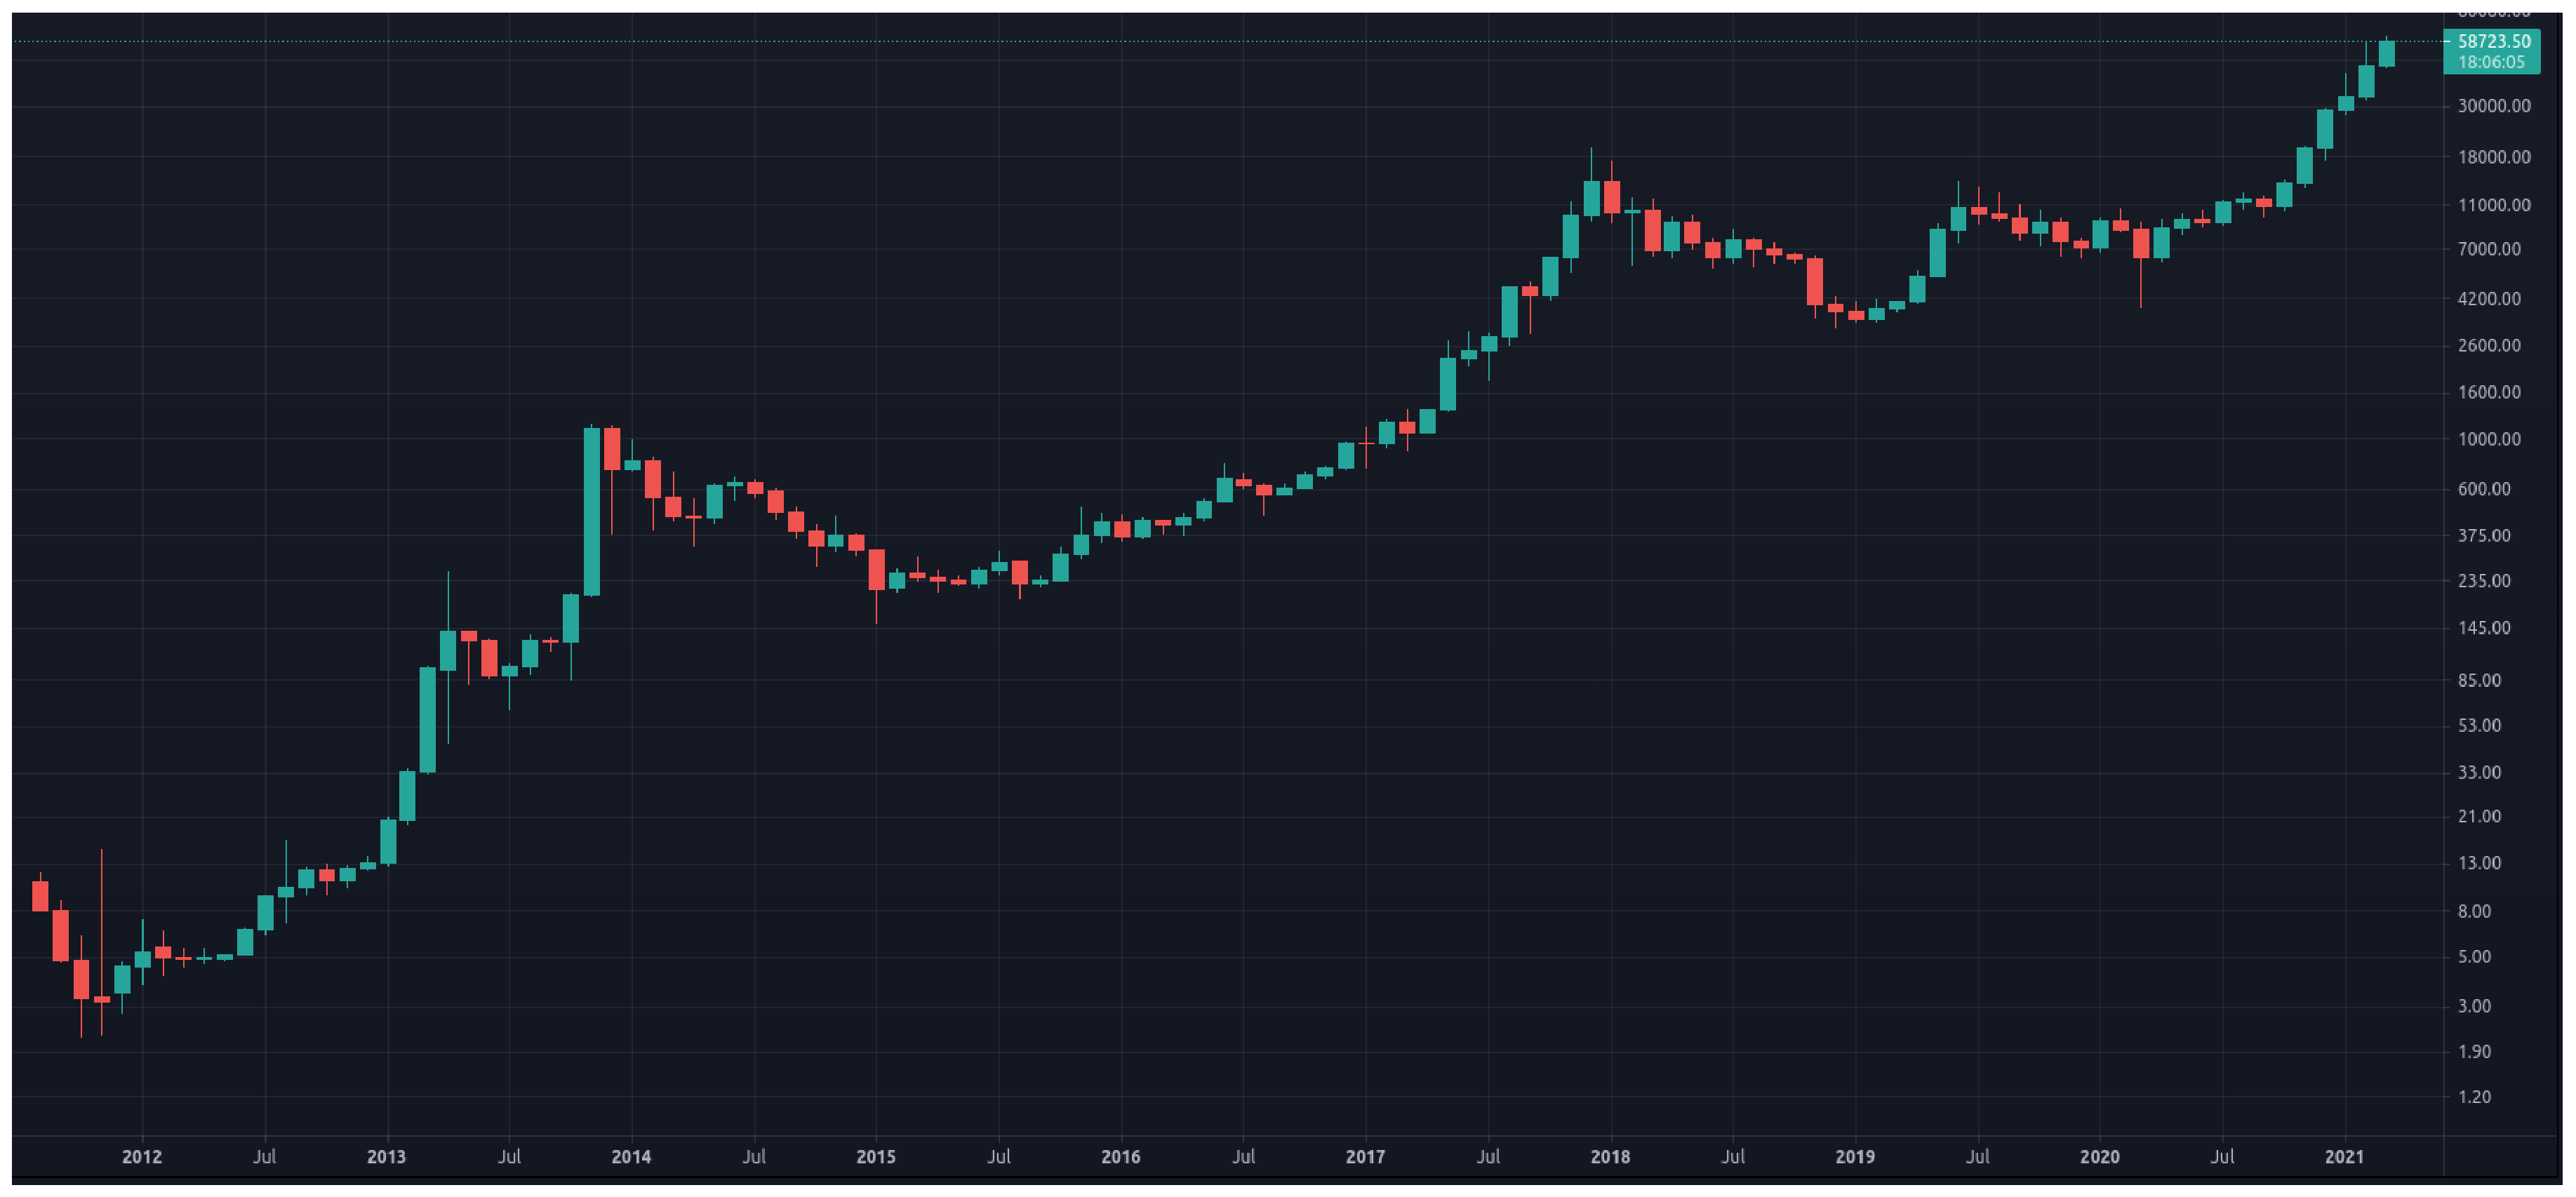
\includegraphics[width=\textwidth]{figs/btusd.eps}
% \caption{BTC/USD}
% \label{fig:btcusd}
%\end{figure}
\begin{figure}
    \centering
    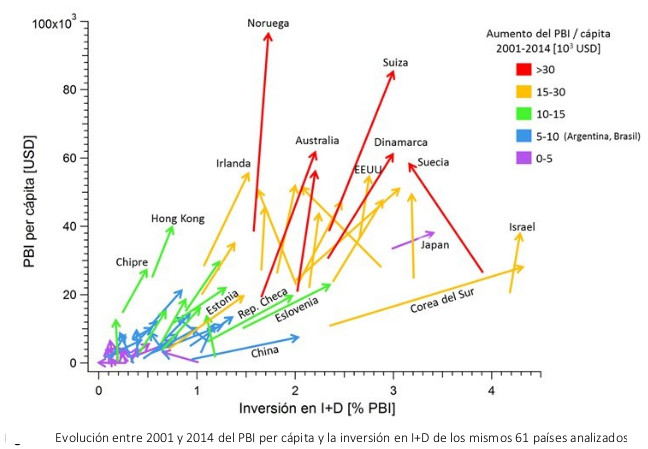
\includegraphics[width=0.5\textwidth]{figs/Docuemnto_Stefani_2.jpg}
    \caption{\href{https://aargentinapciencias.org/wp-content/uploads/2019/05/Docuemnto_Stefani.pdf}{\beamergotobutton{Congressional Report, Prof Stefani}}} 
\end{figure}
\subsection{Indexing Open Production and Development}

If Bitcoin/Blockchain is a decentralized technology, its use as a store-of-value for Astronomy must complement decentralized education, research, and development. This is embodied in its name-sake, so-called term: "Open Development".

A community defined and validated AOD system could be used to evaluate preferred funding channels including node validation via incentives Txn types. Such a system could be periodically revised by the community with community governance protocols that ideally would respect yet complement existing structures in a self-consistent decentralized manner. IVOA could be the perfect example with 19 Nation State member countries and 4 international members. These metrics could be used to direct and supply liquidity for the Open Development of Astronomy. As seen in Fig Seffanni. national governments that spend a larger percentage of GDP towards science and technology also on average have higher GDP growth rates (in USD). So this could be a weighting factor metric. See equtation1. Reciprocal percentage of total GDP towards science could be a constructed normalization parameter. So too could total debt to GDP public debt.  An example is the Maker ERC231 ETH governance token that itself control a  pseudo-decentralized US stable coin bank, DAI, over-collateralised that has remained 1 USD for several years despite the BTC market varience.  On the question of whether a special token need minting. The pros and cons need to be carefully studied by the community. For example WETH and WBTC are stable tokens that are on native ETH but allow interconectivity between chains. A similar system occurs with the price issuance of DAI via Maker. It is an important element of DEFI and governence that is included in Figure 2.   

DEFI protocols and more general community may have some motivation to provide decentralized funding for astronomy Open Development. First, Open development protocols could insure existing methods and procedures mauy also be applicable to the Open Development of Astronomy Community. Both  based on Open Source technology, that follow the Lindy effect.
 
\subsection{Model Attributes of a Token for Astronomy}
\label{subsec:btc4}
There are certainly advantages if the community has its own token. But there are also disadvantages. RSA Ecliptic Curve Algorithm, asymetric hash function, Blind, Schnor Signatures, Merkle Trees, ZKP,  WEB3, Multi-sig, Cross chain, mixing - Privacy. 

\subsection{Block Validation}
\label{subsec: validator}
Blockchain Validators and Nodes. ERC20 Protocalls like GRT ERC   

\href{https://defipulse.com/}{DEFI$\;$ PULSE} pulse is a list of all the liquidity that is tied into DEFI. There is over 77.77 $\times 10^{9}$ USD locked in DEFI. The UNISWAP treasury has in excess of 3 billion dollars. These treasury funds are available via grants programs that Astronomy Open Development protocols should have access to.

In this Section, a toy model for the open development of Astronomy based on open Blockchain technology is presented. An attempt is made to sketch out ingredients and methods of a `successful' model. Some elemental principals as voted by governance should be voted at different stages calibration proposals. For argument sakes in this model we follow the UNISWAP snapshot community, where there are different instances of governance. We also have a treasury funds, and the like.  through governance solutions. The UNISWAP model, to date is one of the largest decentralized exchange, has many developers working for it, was the first massive airdrop token of Blockchain value, so is essentially decentralized in our assumption. The funds for this Paper come from DEFI, from the NOVA node of the IVOA-EXEC committee for Argentina. Some fundamental actors are identified and their functionality with the model sketched out. This paper does not pretend to discuss in strict technical details the finer points of the implementation of such model and parameters therein, but does make reference to some basic cryptographic primatives including Merkle Trees, Zero-knowledge proofs, cross chain protocals, etc. that offer promising solutions and could certainly be considered to be incorporated during Improvement Proposals directed by the community periodically. The paper does not delve into technical details of some Blockchain procedures like mixing to maintain secure personal and private information but of all actors but pretends to highlight some core model features to be followed up by future authors but obviously  locked value will naturally flow to the more useful protocols.  
 
The only condition to participate is bonafide scientific curiosity for Astronomy so sufficient incentive methods need to be developed to entice value-added interaction with the astronomy Blockchain via Decentralized Block Chain Applications, (DAps) as programmable parameters that can be set by the Model's governance component albeit individual minority actors. 

%This part examines a type of Model. The ICO era based on the Ethereum smart contracts bubble that burst aside from rthe egulatory issues about Securities that was mostly based on near useless speculative tokens must be avoided by any AOD bonafide . It looks at some main or speculive  I would not be in favour of an ICO, I think founds are complimentary and as such must come forom existing DEFI protocol pools. But the Community must decide this. However, For the sake of simplicity the following three `actors' are identified as founding governance members: International Virtual Observatory Alliance, the  Astropy community and authors of referred peer reviewed journals weighted by their h-index, the International Astronomy Union etc. Parameters such as the weight of each should be set soon and be discussed by the community and there could even be a switch or that must be voted on according to community established acoords. For example astropy community. A type of switch could be voted for to change the relative percentage of votes.UNISWAP for exmaple is the first governence token that inclduded the AMM liquidity  The reward will be the AstroOD Token, since the wallet creation, Blockchain exploder and DApp python tools and protocols are unified by the proposed affiliated package of astropy. This parameter could be considered to as a proportionality of any initial coin distribution function. But we would be against this and think programs need to start from the ground-roots up, providing liquidity and rewarding Tx were useful (community validaded) Tx occur. On Balance an initial token distribution or ICO has drawbacks and so our model draws on existing liquidity pools from the DEFI Space.

Over 70 percent of Astronomers use  Astropy and recent paper in preparation show a promising metric in developer community as the community developer toolkit for Open Source code, that with VO software makes up the majority toolkit of astronomers barring some HPC computing for N-body simulations. Many astronomers probably agree to say these would be the recognized go-to  Astronomy Software and Development so the Astropy Community onboarding, usefulness would be advantages to the Open Development Astronomy model (here-after ODM) of Astronomy as proposed. Affiliated package authors could be validated and offered a period to open a wallet and partake in governence DAO. An affiliated package to Astropy is selected to generate private public SHA256 pairs and the generated funds will be locked by the Community 70 percent to Developers. 

No initial coin offering is neesary as this would be deemed a securtiy and may violate some Legal Juristicitions that we argue for Open Development must be lawful yet, at the same time decentralized means if a majority want and if safeguards are put in place, ie truelly decnentralized nodes, not INFURA WEB three but above. So recognizing `challanges' that Open Protocol must face and converging on Wrights Law of the CDF of Astronomy Developement we appeal to DEFI grant protocols to fund our development. 


The AstroOD package 

We propose an AstroOD coordinated package \textcolor{red} github ref. that periodically receives data-feeds on AstroOD on collects basic statistics of packages being used and is correlated to ADS Main-Text query and ORCID query. A possibility is to build a SubGraph to program as an Oracle on UNISWAP. UNISWAP liquidity    Anyone in the Astropy community can create key pairs to be used as Smart Contract accounts. The program using RSA, and blind signature for privacy. The package will include a functional wallet, with multi signature, multi currency and multiple accounts. This will be the basis of deployment of “Smart Contracts”, as a concept was introduced in 1995 by Nick Szabo, who described Smart Contracts as “a set of promises,
specified in digital form, including protocols within which these parties perform.

AstroOD package will have to be built to implement the use of Oracles, to connect the community to the Blockchain space. Oracles manage feeds of information are not put into the native Blockchain due to scalability or privacy issues, etc but to other Chains.  Oracles are more focused on price-feed data for crypto asset prediction markets but with DEFI burgeoning and necessity the Oracle inputs are becoming more diversified.  The Oracle Problem 4 promises” (Szabo, 1996). 

Feeds for Oracles would include ADS-NASA, ArchieX ., etc,  to validate information that can be used to automatically set parameters in the model. The weights could be voted on by IVOA representatives.

If the  model truly represents an open Blockchain then anyone can participate and be offered rewards as incentive in pursuit of open astronomy. It is obviously important that protocol standards be defined and a body like IVOA could be instrumental in helping to define them with the Astropy community, for example. That body could take into account validaded economic considerations like inflation of national currencies., crisis, etc. Staked AstroOD tokens can be awarded using a 'competative' awards scheme program to Secondary School Teachers, Plenetarium guides, thesis graduate students etc. that work to teach astronomy. All must have oportunity to receive incentive rewards for their valid contributions including for example validated University students and volunteers that mount Open-Day/Night activity for the public, etc., All should receive incentive rewards for their contribution since sacrificing their time in sharing knowledge to allow others opportunities should be rewarded as it is clearly in pursuit of Open Development. Weightings for these activities can be set periodically by the governance component with mandatory revision periods, and clauses if they change too abruptly. An option is to follow MakerDAO governance models, with funds from Treasury. Unfortunately political, financial, health  crisis cause by rampant financial speculation and the like, will probably not be solved by Central Bank Digital Currencies, as these are essentially still centralised institutions on a Blockchain.  Often during these crisis outreach and educational activities are the first casualty of open development, as are essential and scares resources for Public University and National Institute research bodies. In the case of the creation of events, the governance model will award staked token holder to provide credit for future open development. Authors who publish papers also may claim awarded tokens and trade them too?

\subsection{Digital Open Ledger Technology}

\subsection{ERC 721 }

ERC 721 tokens are an ETH standard token contracts that are Non-Fungible Token (NFT), ie they are unique and indivisible or in other words can be used to identify a unique event, object or condition. This type of Token may be used on platforms that offer digital collectibles, access keys, lottery tickets, numbered seats for concerts, sports matches or academic meetings, for example best "student" poster prizes in conferences, etc. 

ERC 721 tokens may have different values from one another although derived from the same Smart Contract base, due to its age, rarity often iconized by its unique visual artistry (appearance).

The uint256 variable or called tokenId, so for any ERC-721 Contract, the pair contract address, uint256 tokenId must be globally unique. Said that a dApp can have a "converter" that uses the tokenId as input and outputs an image of something cool, like zombies, weapons, skills or amazing kitties!


With PAOP protocol ERC721 SMart Contract Non-Fungable Tokens can be issued on demand if needbe. These digital collectables will be sold on a Dex funded exchange, to provide liquidity to further Scientific-Cultural use-case.

i) A PhD scholarship holder has run out of PhD Funding 
ii) A Group that is working in some country has had the USD devalued and the subsidy payments are late, and they are applying for some tokens and offer in exchange a collaborate NFT to be published in the acknolodgements of the paper.
iii) A group of astronomers, technicians, students,  are building an observatory in a advantageous site in a poor country. 

\subsection{Tokenisation}

Since centralized regulation that at some stage may undermine public open Blockchain science development and by weighing-up pros/cons between POW and POS consusus, of the Table blockpros/cons as well as from recognizing the 12 year dominance of BITCOIN we choose to follow governance model tokenisation, adopted by  companies like "Shape-Shift" a XXX billion USD companies that has become completely Tokenized. Any system must be able tp use Bridges even to different chains. 

Its xxx workers were each given some tokens as where select members from the community. 

A possible route of course is to solicit an initial token grant from UNI the largest decentralized exchange provider as well as other DEFI DAOs, then in an active campaign period leading up to the token release allow for initial KYC. Since We need to validate some key actors that include students that are doing a graduate or undergraduate degree with major in Astronomy professors of Astronomy Univsersity Courses. Developers, authors and co-authors of open development astronomical software, including those of affiliated packages in Astropy. 

\subsection{Initial Token Distribution}
#This part so far just fun ideas but not so in favour of having an ILO or ICO etc., thinking the CONS are to stacked up against it but eventually 
Authors and co-authors Via the MNRAS sites and some form of Zero Knowledge Proof Validation will be able for each paper publishes list astroOD, that will be obtained from Treasury.

\subsection{Liquidity pools}

Liquidity pools for Astronomers , Travel Conferences, Observing, Teaching, these pools can be flexible but it is advised to be a percentage of PhD  students or some metric related to PhDs produced. 

\subsection{Career Development in Astronomy}

Over the time-scale of 5 years, incidentally about the average time it takes a new astronomy major to complete a PhD, the Ethereum and Bitcoin Blockchain's have stood-up to their promise to hold store of value. See Figure 1 and 2. These Bitcoin and Ethereum Blockchains did not implode during the March 2020 flash-crash, probably motivated investors to seek liquidity across all markets in a COVID19 inspired pullback of main street.  Bitcoin ref(Satoshi Nakamoto) was born to be a store of value after the 2008 sub-prime morgage backed securities, credit default swap fiasco when the worlds largest banks were called to account causing the greatest financial crisis since the great depression of 1930's and is standing up now, when the FED, the US treasury and some central banks have offered to emit as much money as it takes to.
 
In this context it should be of no surprise that the Argentina Gemini membership in 2020 may even be under-threat depending on what the consorsium decides on behalf of Argentina. A situation since only a small fraction of the funds required for 2019 were delivered by the previous government and astronomers wages and subsidies are perceived to be undervalued. Unfortunately the news for science in general was not so great since the Ministry of Science was disbanded and funding to host international conferences in 2019 was put on a stand still. Although the new government did fund a new Ministry for Science, and Blockchain technology is considered a strategic area, there is actual little technology being adopted. If adequate funding is not forthcoming this could still signify retract in the educational scientific and technological potential of Argentina as an emerging country including a new brain drain wave for young-scientists, as talent settles overseas. 

This dire context above was contracted in complicity with loan requirements, exerted by the International Monetary Fund through loan obligations/conditioning that prioritized a creditor bonanza scheme based on a 70\% bank lending rate set by the PRO party coalition led by the ex-president of Paradise Paper's acclaim that ran a coalition government to full-term. 

Underlying this debt ridden situation, is a loaming world recession within a COVID-19 pandemic context with the cancellation of international Astronomical conferences, workshops and other meetings is taking place at a global scale: IVOA suspended its May Sydney Interop meeting and in Argentina the Observatory Astronomical of Cordoba (circa 1873) one of the first national scientific institutions with the Instituto de Astronomia Teorica y Experimental announced the suspension of the 2021 Friends of Friends workshop. 

It is argued that the current crisis, like the last major one that affected the research capacity of scientisits to conduct their work in Argentina was the 2001 economic crisis, when Argentina paid for being the "poster child of the IMF" with the greatest default in history and before that, when the Argentina Scientific output capacity was being determined down the barrel of a gun by the military junta and some home-grown scientists that would probably prefer to stay unnamed that seeminlgy justified this collateral damage (see Nature Levato paper, that was arrested in what appears a Mysogenic probably unrelated case.

In this context and given the fact that the half-life rate of Astronomy majors from US public universities has been in steep free-fall.  \cite{milo_2018} it is that the discussion of incentivizing using Blockchain tokenomics. At the same time, government spending in the military industrial complex, banks, insurer and corporate bail-outs are at an all time high so as scientist it could be argued that it is our responsibility to add checks and balances with recognizably proven community technology. 
%
If such a model exists it is certain that data Feeds protocols will become an important part to allow to mitigate mistakes from central actors since the system must be largely transparent yet private when it needs to be. Our model would use Zero Knowledge Proofs and other Blockchain primitives to safe-guard privacy of information of the individual yet also compensate or incentives the brave. 
   
The identification of elements or properties for the programmatic `tokenization' of an open development protocol for astronomy should not be limited or influenced by any one central authority or by the political economy of any one partner of IVOA or any other nation and should be based heavily on open source praxis paradigm. 
   
In Section INTRO we stated the motive and underlying potential of applying open development technology to astronomy. We detail with warp speed some crytographic primitives (Has functions, Merkle roots) and some basic protocols to establish a general model frame-work of Tokenomics, including staking or yield-farming incentive mechanics, time and value locked development fund release functions, and also discuss the implications of governance, etc,

\section{Use-case for Decentralized Finance}
\label{sec:use-case}

Liquidity is a necessary resource of any token model. Our Open Development Model requires liquidity. The patch offered here is to tie into the liquidity pools of the decentralized finance movement that we would hope to form a common token fund. Some parameters of the funding rate, principally by UNISWAP grant, would be determined by that community.   

\section{Case-Study}
\label{sec:btc5}

\begin{itemize}
    \item{SSO SSS defence contractor that had previously developed ordnance systems on weapons that served in the Illegal war in Iraq was knowingly selected to build the Sky-Mapper detector. } 
    \item{NSF Shutdown or Telescopes in EEUU during Obama and Trump administrations}
    \item{Split decision of the Australian community under the Hawke government to direct funds to upgrade of radio-facilities in Australia, instead of ESO membership}
    \item{Close door period of Scientific Research position in Argentina, 1990's}
    \item{Gemini contractual issue for Argentina, implicating a withdraw of funding from the ministry of funding, and a divided community because of recommended reduction of Gemini time.}
    \item{NFT for the MOA}, see Figure 1, which the Astronomical Observatory of Cordoba holds NFT ownership and wishes to sell for to help fund the MOA and research activities. 

\end{itemize}


\section{Decentralized Finance} 

Case study of NFT
\begin{figure}[h!]
    \centering
    \label{fig:my_label}
  \caption{NFT collectable, world event to constrain Einstein's GTR before publication, foto by the C\'ordoba Observatory team,
during the 1912 eclipse expedition. The Perrine settlement is located in the right, attached to the big white building. Courtesy of the Museo Astron\'omico del Observatorio Astron\'omico de C\'ordoba, C\'ordoba, Argentina.}
  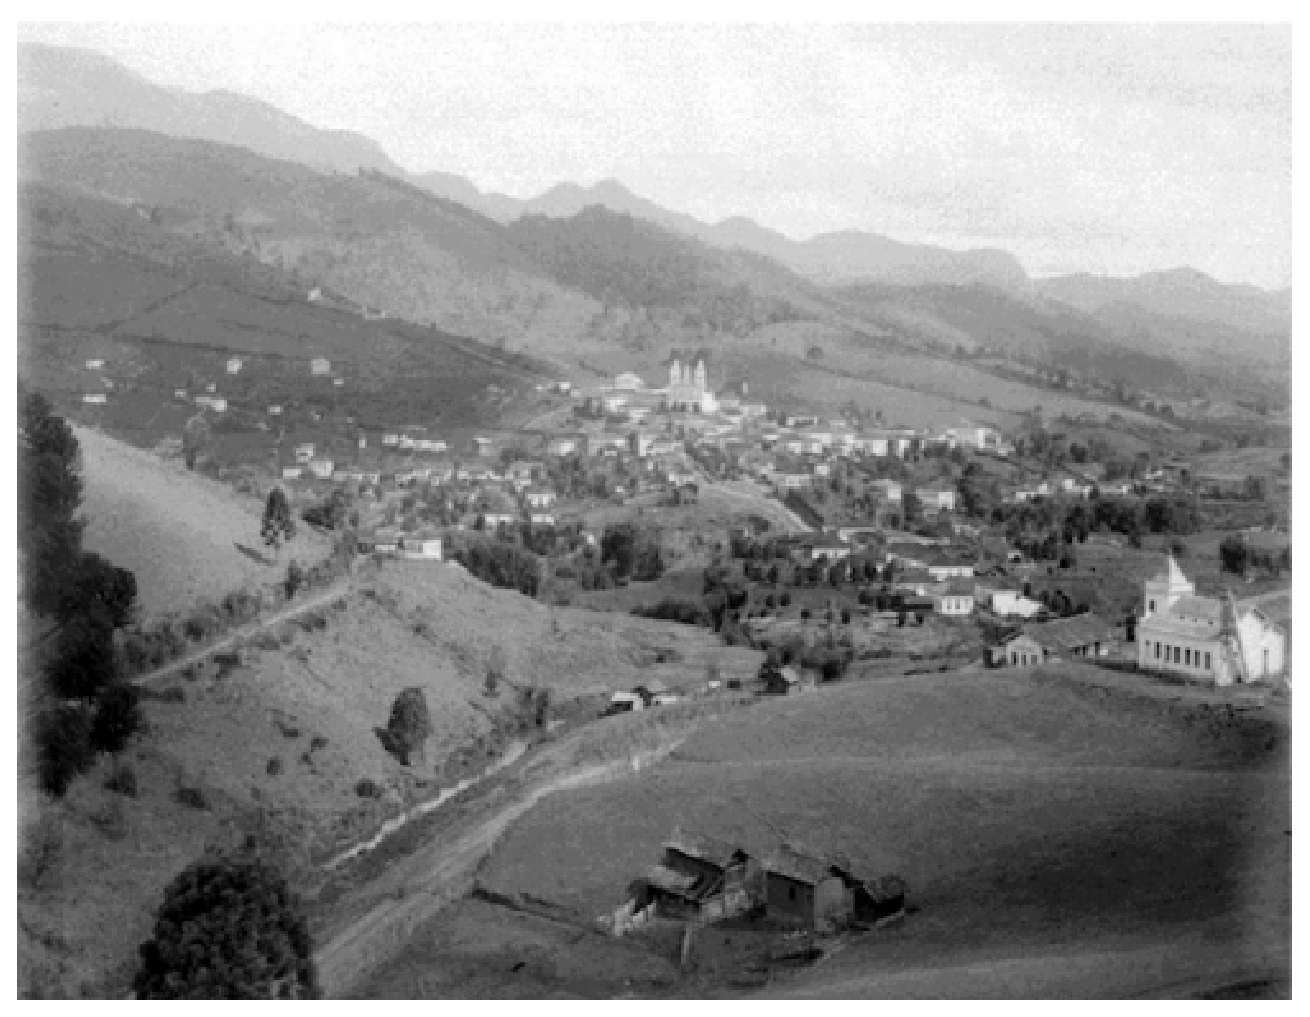
\includegraphics[width=0.4\textwidth]{figs/p1912.eps}
\end{figure}



% =============================================================================
% Smart Contracts
% =============================================================================
\section{Context}
\label{section:context}
%


% =============================================================================
% POAP.xyz
% =============================================================================
\section{Developer tools}
\label{section:Eth721}
%
We consider that since astropy is the leading open developer toolkit for astronomical research reflected in the astropy  user and dev comits see \cite{ 2020ASPC..522..491T}, that it be used at t0 launchdate but details could even be revised later by governance.  The Etherium Blockchain contains a type of smart contracts called NFT or non-fungable token.  This type of token is non-interchangable can be unique to preserve the notion of digital scarcity, and can be verified without any centralized organization required to authenticate it. These smart contracts can be used issue incentive rewards to nodes. A protocol build around 721 protocal includes POAP.xyz, ref(github address). This proof of attendance protcol can be used to validad the attendance of astronomical events, including virtual ones. The tokens can be exchanged for goods and services and soldon for fiat money.  


Data feeds will be entered into Oracles that will automatically via smart contracts provide incentive rewards to the node and user wallets.
%
POAP type proof of attendence protocol for meetings. To rewards students for attending and presenting their results in meetings.
%
\subsection{Hash Function Account}
We propose for any developer of Astropy core plus afiliated package models including co-authors are onboarded and in our model we apply the afilated package astropy Package astrobtc, recognizing the fact that Bitcoin has been the major asset class for the last 12 years that included several global crisis. 
%

Astropy proving to revolutionize astronomical data-reduction collaboration and is channelled through the open development of astronomy project Astropy. It involves IVOA's 20 member institution was originally much smaller and conceived by its founding members to be a large fraternal virtual observatory working seamlessly in perfect collaboration with no imposed boundaries other than those of the ethical nature. Today it consists of mostly national VO members as well as three very important international members that include: the European Space Agency, the European VO and the UK VO. The national members are: Argentina, Armenia, Australia, Brazil, Canada, China, \textit{Europe}, France, Germany, Hungary, India, Italy, Japan, Korea, Russia, Spain, Ukraine, the United Kingdom and the United States. This `paper' proposes to open the discussion on the adoption of Block-chain technology for IVOA for the open development of astronomy. It is written in the context of long term flaws experienced in the current development model paradigm that results in less than efficient research inventive mechanism and cyclic funding crisis as well as possibly serendipitous COVID-19 type pandemic that may become more frequent.
%
Aside from some issues as illustrated below that would pausibly affects any 'closed' development model for astronomy, or one determined by powerful central actors, one based on open Blockchain technology should, on the other hand preferable gravitate to real open development via carefully thought-out and implemented incentive mechanisms to foster collaboration in a more efficient way and lay the path to unprecedented scientific discovery and innovation. It is in this context that I invite the reader to contemplate on the opening discussion of IVOA in the field of tokenomics. 
%
Our analysis focuses on the US public university research system, some limited experience on the IVOA system and the Argentine, Australian astronomical research system. 
   
   Strong motivation for this discussion is based on the facts that:
   
\begin{itemize}
       \item A dwindling half-life for the Astronomy and astrophysics PhD majors in US, Australian \& British (etc,) public university system meaning astronomy and astrophysics is loosing a main investment, its researchers.  
       
       \item Shortfalls caused by ciclic funding crisis that affect education institutions, scientific research facilities observed as acute funding restrictions, cutbacks and "government shutdowns" and/or inflation in national currencies, is the elephant in the room that must be addressed.
\end{itemize}
       
       
This paper argues the use of "Blockchain Technology" as a necesarry tool for efficient and sustainable open development in Astronomy as an underlying incentive mechanism for collaboraborative research projects that foster open development community identified metrix.  


% =============================================================================
% SECTION CONCLUSIONS
% =============================================================================
\section{Conclusions and Future Work}
\label{sec:5}
%
In this study, we set ourselves a task to discuss systemic issues that have hampered Open Development for Astronomy and propose an affiliated package to astropy AstroOD to build on the DEFI stack including the creation of wallets. This new package is required to be developed by the community and must be compatible with up-coming Python versions and be fully documented in a public repository. 
%
Future development will focus on the following three areas: incorporating
new features, improving documentation, and 
possible integration with tools for interactively analyzing features of development.

IAU and IVOA Astronomer data-base to validate loose KYC, coordinating contact with institutions. 

% =============================================================================
% SECTION Acknowledgments
% =============================================================================
\section{Acknowledgments}
SG acknowledges the New Virtual Observatory of Argentina (NOVA) and his selection as representative of Argentina on the IVOA-exec committee.

% =============================================================================
% SECTION BIBLIO
% =============================================================================
%
%\section*{References}
%\label{biblio}
\bibliographystyle{model2-names-astronomy}
\bibliography{ivoatoken}


\end{document}

\endinput